
% Default to the notebook output style

    


% Inherit from the specified cell style.




    
\documentclass[11pt]{article}

    
    
    \usepackage[T1]{fontenc}
    % Nicer default font (+ math font) than Computer Modern for most use cases
    \usepackage{mathpazo}

    % Basic figure setup, for now with no caption control since it's done
    % automatically by Pandoc (which extracts ![](path) syntax from Markdown).
    \usepackage{graphicx}
    % We will generate all images so they have a width \maxwidth. This means
    % that they will get their normal width if they fit onto the page, but
    % are scaled down if they would overflow the margins.
    \makeatletter
    \def\maxwidth{\ifdim\Gin@nat@width>\linewidth\linewidth
    \else\Gin@nat@width\fi}
    \makeatother
    \let\Oldincludegraphics\includegraphics
    % Set max figure width to be 80% of text width, for now hardcoded.
    \renewcommand{\includegraphics}[1]{\Oldincludegraphics[width=.8\maxwidth]{#1}}
    % Ensure that by default, figures have no caption (until we provide a
    % proper Figure object with a Caption API and a way to capture that
    % in the conversion process - todo).
    \usepackage{caption}
    \DeclareCaptionLabelFormat{nolabel}{}
    \captionsetup{labelformat=nolabel}

    \usepackage{adjustbox} % Used to constrain images to a maximum size 
    \usepackage{xcolor} % Allow colors to be defined
    \usepackage{enumerate} % Needed for markdown enumerations to work
    \usepackage{geometry} % Used to adjust the document margins
    \usepackage{amsmath} % Equations
    \usepackage{amssymb} % Equations
    \usepackage{textcomp} % defines textquotesingle
    % Hack from http://tex.stackexchange.com/a/47451/13684:
    \AtBeginDocument{%
        \def\PYZsq{\textquotesingle}% Upright quotes in Pygmentized code
    }
    \usepackage{upquote} % Upright quotes for verbatim code
    \usepackage{eurosym} % defines \euro
    \usepackage[mathletters]{ucs} % Extended unicode (utf-8) support
    \usepackage[utf8x]{inputenc} % Allow utf-8 characters in the tex document
    \usepackage{fancyvrb} % verbatim replacement that allows latex
    \usepackage{grffile} % extends the file name processing of package graphics 
                         % to support a larger range 
    % The hyperref package gives us a pdf with properly built
    % internal navigation ('pdf bookmarks' for the table of contents,
    % internal cross-reference links, web links for URLs, etc.)
    \usepackage{hyperref}
    \usepackage{longtable} % longtable support required by pandoc >1.10
    \usepackage{booktabs}  % table support for pandoc > 1.12.2
    \usepackage[inline]{enumitem} % IRkernel/repr support (it uses the enumerate* environment)
    \usepackage[normalem]{ulem} % ulem is needed to support strikethroughs (\sout)
                                % normalem makes italics be italics, not underlines
    

    
    
    % Colors for the hyperref package
    \definecolor{urlcolor}{rgb}{0,.145,.698}
    \definecolor{linkcolor}{rgb}{.71,0.21,0.01}
    \definecolor{citecolor}{rgb}{.12,.54,.11}

    % ANSI colors
    \definecolor{ansi-black}{HTML}{3E424D}
    \definecolor{ansi-black-intense}{HTML}{282C36}
    \definecolor{ansi-red}{HTML}{E75C58}
    \definecolor{ansi-red-intense}{HTML}{B22B31}
    \definecolor{ansi-green}{HTML}{00A250}
    \definecolor{ansi-green-intense}{HTML}{007427}
    \definecolor{ansi-yellow}{HTML}{DDB62B}
    \definecolor{ansi-yellow-intense}{HTML}{B27D12}
    \definecolor{ansi-blue}{HTML}{208FFB}
    \definecolor{ansi-blue-intense}{HTML}{0065CA}
    \definecolor{ansi-magenta}{HTML}{D160C4}
    \definecolor{ansi-magenta-intense}{HTML}{A03196}
    \definecolor{ansi-cyan}{HTML}{60C6C8}
    \definecolor{ansi-cyan-intense}{HTML}{258F8F}
    \definecolor{ansi-white}{HTML}{C5C1B4}
    \definecolor{ansi-white-intense}{HTML}{A1A6B2}

    % commands and environments needed by pandoc snippets
    % extracted from the output of `pandoc -s`
    \providecommand{\tightlist}{%
      \setlength{\itemsep}{0pt}\setlength{\parskip}{0pt}}
    \DefineVerbatimEnvironment{Highlighting}{Verbatim}{commandchars=\\\{\}}
    % Add ',fontsize=\small' for more characters per line
    \newenvironment{Shaded}{}{}
    \newcommand{\KeywordTok}[1]{\textcolor[rgb]{0.00,0.44,0.13}{\textbf{{#1}}}}
    \newcommand{\DataTypeTok}[1]{\textcolor[rgb]{0.56,0.13,0.00}{{#1}}}
    \newcommand{\DecValTok}[1]{\textcolor[rgb]{0.25,0.63,0.44}{{#1}}}
    \newcommand{\BaseNTok}[1]{\textcolor[rgb]{0.25,0.63,0.44}{{#1}}}
    \newcommand{\FloatTok}[1]{\textcolor[rgb]{0.25,0.63,0.44}{{#1}}}
    \newcommand{\CharTok}[1]{\textcolor[rgb]{0.25,0.44,0.63}{{#1}}}
    \newcommand{\StringTok}[1]{\textcolor[rgb]{0.25,0.44,0.63}{{#1}}}
    \newcommand{\CommentTok}[1]{\textcolor[rgb]{0.38,0.63,0.69}{\textit{{#1}}}}
    \newcommand{\OtherTok}[1]{\textcolor[rgb]{0.00,0.44,0.13}{{#1}}}
    \newcommand{\AlertTok}[1]{\textcolor[rgb]{1.00,0.00,0.00}{\textbf{{#1}}}}
    \newcommand{\FunctionTok}[1]{\textcolor[rgb]{0.02,0.16,0.49}{{#1}}}
    \newcommand{\RegionMarkerTok}[1]{{#1}}
    \newcommand{\ErrorTok}[1]{\textcolor[rgb]{1.00,0.00,0.00}{\textbf{{#1}}}}
    \newcommand{\NormalTok}[1]{{#1}}
    
    % Additional commands for more recent versions of Pandoc
    \newcommand{\ConstantTok}[1]{\textcolor[rgb]{0.53,0.00,0.00}{{#1}}}
    \newcommand{\SpecialCharTok}[1]{\textcolor[rgb]{0.25,0.44,0.63}{{#1}}}
    \newcommand{\VerbatimStringTok}[1]{\textcolor[rgb]{0.25,0.44,0.63}{{#1}}}
    \newcommand{\SpecialStringTok}[1]{\textcolor[rgb]{0.73,0.40,0.53}{{#1}}}
    \newcommand{\ImportTok}[1]{{#1}}
    \newcommand{\DocumentationTok}[1]{\textcolor[rgb]{0.73,0.13,0.13}{\textit{{#1}}}}
    \newcommand{\AnnotationTok}[1]{\textcolor[rgb]{0.38,0.63,0.69}{\textbf{\textit{{#1}}}}}
    \newcommand{\CommentVarTok}[1]{\textcolor[rgb]{0.38,0.63,0.69}{\textbf{\textit{{#1}}}}}
    \newcommand{\VariableTok}[1]{\textcolor[rgb]{0.10,0.09,0.49}{{#1}}}
    \newcommand{\ControlFlowTok}[1]{\textcolor[rgb]{0.00,0.44,0.13}{\textbf{{#1}}}}
    \newcommand{\OperatorTok}[1]{\textcolor[rgb]{0.40,0.40,0.40}{{#1}}}
    \newcommand{\BuiltInTok}[1]{{#1}}
    \newcommand{\ExtensionTok}[1]{{#1}}
    \newcommand{\PreprocessorTok}[1]{\textcolor[rgb]{0.74,0.48,0.00}{{#1}}}
    \newcommand{\AttributeTok}[1]{\textcolor[rgb]{0.49,0.56,0.16}{{#1}}}
    \newcommand{\InformationTok}[1]{\textcolor[rgb]{0.38,0.63,0.69}{\textbf{\textit{{#1}}}}}
    \newcommand{\WarningTok}[1]{\textcolor[rgb]{0.38,0.63,0.69}{\textbf{\textit{{#1}}}}}
    
    
    % Define a nice break command that doesn't care if a line doesn't already
    % exist.
    \def\br{\hspace*{\fill} \\* }
    % Math Jax compatability definitions
    \def\gt{>}
    \def\lt{<}
    % Document parameters
    
\title{Chapter 2: Damped Harmonic Oscillators}

    
\date{11 and 14 September 2017}

    
\author{Nicolas Grisouard, nicolas.grisouard@physics.utoronto.ca}

    

    % Pygments definitions
    
\makeatletter
\def\PY@reset{\let\PY@it=\relax \let\PY@bf=\relax%
    \let\PY@ul=\relax \let\PY@tc=\relax%
    \let\PY@bc=\relax \let\PY@ff=\relax}
\def\PY@tok#1{\csname PY@tok@#1\endcsname}
\def\PY@toks#1+{\ifx\relax#1\empty\else%
    \PY@tok{#1}\expandafter\PY@toks\fi}
\def\PY@do#1{\PY@bc{\PY@tc{\PY@ul{%
    \PY@it{\PY@bf{\PY@ff{#1}}}}}}}
\def\PY#1#2{\PY@reset\PY@toks#1+\relax+\PY@do{#2}}

\expandafter\def\csname PY@tok@sd\endcsname{\let\PY@it=\textit\def\PY@tc##1{\textcolor[rgb]{0.73,0.13,0.13}{##1}}}
\expandafter\def\csname PY@tok@s2\endcsname{\def\PY@tc##1{\textcolor[rgb]{0.73,0.13,0.13}{##1}}}
\expandafter\def\csname PY@tok@kr\endcsname{\let\PY@bf=\textbf\def\PY@tc##1{\textcolor[rgb]{0.00,0.50,0.00}{##1}}}
\expandafter\def\csname PY@tok@gi\endcsname{\def\PY@tc##1{\textcolor[rgb]{0.00,0.63,0.00}{##1}}}
\expandafter\def\csname PY@tok@go\endcsname{\def\PY@tc##1{\textcolor[rgb]{0.53,0.53,0.53}{##1}}}
\expandafter\def\csname PY@tok@sr\endcsname{\def\PY@tc##1{\textcolor[rgb]{0.73,0.40,0.53}{##1}}}
\expandafter\def\csname PY@tok@sa\endcsname{\def\PY@tc##1{\textcolor[rgb]{0.73,0.13,0.13}{##1}}}
\expandafter\def\csname PY@tok@sh\endcsname{\def\PY@tc##1{\textcolor[rgb]{0.73,0.13,0.13}{##1}}}
\expandafter\def\csname PY@tok@kt\endcsname{\def\PY@tc##1{\textcolor[rgb]{0.69,0.00,0.25}{##1}}}
\expandafter\def\csname PY@tok@o\endcsname{\def\PY@tc##1{\textcolor[rgb]{0.40,0.40,0.40}{##1}}}
\expandafter\def\csname PY@tok@nn\endcsname{\let\PY@bf=\textbf\def\PY@tc##1{\textcolor[rgb]{0.00,0.00,1.00}{##1}}}
\expandafter\def\csname PY@tok@gp\endcsname{\let\PY@bf=\textbf\def\PY@tc##1{\textcolor[rgb]{0.00,0.00,0.50}{##1}}}
\expandafter\def\csname PY@tok@cp\endcsname{\def\PY@tc##1{\textcolor[rgb]{0.74,0.48,0.00}{##1}}}
\expandafter\def\csname PY@tok@se\endcsname{\let\PY@bf=\textbf\def\PY@tc##1{\textcolor[rgb]{0.73,0.40,0.13}{##1}}}
\expandafter\def\csname PY@tok@mf\endcsname{\def\PY@tc##1{\textcolor[rgb]{0.40,0.40,0.40}{##1}}}
\expandafter\def\csname PY@tok@sc\endcsname{\def\PY@tc##1{\textcolor[rgb]{0.73,0.13,0.13}{##1}}}
\expandafter\def\csname PY@tok@mh\endcsname{\def\PY@tc##1{\textcolor[rgb]{0.40,0.40,0.40}{##1}}}
\expandafter\def\csname PY@tok@kn\endcsname{\let\PY@bf=\textbf\def\PY@tc##1{\textcolor[rgb]{0.00,0.50,0.00}{##1}}}
\expandafter\def\csname PY@tok@gt\endcsname{\def\PY@tc##1{\textcolor[rgb]{0.00,0.27,0.87}{##1}}}
\expandafter\def\csname PY@tok@mb\endcsname{\def\PY@tc##1{\textcolor[rgb]{0.40,0.40,0.40}{##1}}}
\expandafter\def\csname PY@tok@il\endcsname{\def\PY@tc##1{\textcolor[rgb]{0.40,0.40,0.40}{##1}}}
\expandafter\def\csname PY@tok@gd\endcsname{\def\PY@tc##1{\textcolor[rgb]{0.63,0.00,0.00}{##1}}}
\expandafter\def\csname PY@tok@ow\endcsname{\let\PY@bf=\textbf\def\PY@tc##1{\textcolor[rgb]{0.67,0.13,1.00}{##1}}}
\expandafter\def\csname PY@tok@nl\endcsname{\def\PY@tc##1{\textcolor[rgb]{0.63,0.63,0.00}{##1}}}
\expandafter\def\csname PY@tok@gu\endcsname{\let\PY@bf=\textbf\def\PY@tc##1{\textcolor[rgb]{0.50,0.00,0.50}{##1}}}
\expandafter\def\csname PY@tok@mi\endcsname{\def\PY@tc##1{\textcolor[rgb]{0.40,0.40,0.40}{##1}}}
\expandafter\def\csname PY@tok@err\endcsname{\def\PY@bc##1{\setlength{\fboxsep}{0pt}\fcolorbox[rgb]{1.00,0.00,0.00}{1,1,1}{\strut ##1}}}
\expandafter\def\csname PY@tok@w\endcsname{\def\PY@tc##1{\textcolor[rgb]{0.73,0.73,0.73}{##1}}}
\expandafter\def\csname PY@tok@no\endcsname{\def\PY@tc##1{\textcolor[rgb]{0.53,0.00,0.00}{##1}}}
\expandafter\def\csname PY@tok@s\endcsname{\def\PY@tc##1{\textcolor[rgb]{0.73,0.13,0.13}{##1}}}
\expandafter\def\csname PY@tok@si\endcsname{\let\PY@bf=\textbf\def\PY@tc##1{\textcolor[rgb]{0.73,0.40,0.53}{##1}}}
\expandafter\def\csname PY@tok@kp\endcsname{\def\PY@tc##1{\textcolor[rgb]{0.00,0.50,0.00}{##1}}}
\expandafter\def\csname PY@tok@vi\endcsname{\def\PY@tc##1{\textcolor[rgb]{0.10,0.09,0.49}{##1}}}
\expandafter\def\csname PY@tok@nv\endcsname{\def\PY@tc##1{\textcolor[rgb]{0.10,0.09,0.49}{##1}}}
\expandafter\def\csname PY@tok@cpf\endcsname{\let\PY@it=\textit\def\PY@tc##1{\textcolor[rgb]{0.25,0.50,0.50}{##1}}}
\expandafter\def\csname PY@tok@nc\endcsname{\let\PY@bf=\textbf\def\PY@tc##1{\textcolor[rgb]{0.00,0.00,1.00}{##1}}}
\expandafter\def\csname PY@tok@mo\endcsname{\def\PY@tc##1{\textcolor[rgb]{0.40,0.40,0.40}{##1}}}
\expandafter\def\csname PY@tok@ss\endcsname{\def\PY@tc##1{\textcolor[rgb]{0.10,0.09,0.49}{##1}}}
\expandafter\def\csname PY@tok@gs\endcsname{\let\PY@bf=\textbf}
\expandafter\def\csname PY@tok@cs\endcsname{\let\PY@it=\textit\def\PY@tc##1{\textcolor[rgb]{0.25,0.50,0.50}{##1}}}
\expandafter\def\csname PY@tok@vm\endcsname{\def\PY@tc##1{\textcolor[rgb]{0.10,0.09,0.49}{##1}}}
\expandafter\def\csname PY@tok@ni\endcsname{\let\PY@bf=\textbf\def\PY@tc##1{\textcolor[rgb]{0.60,0.60,0.60}{##1}}}
\expandafter\def\csname PY@tok@vg\endcsname{\def\PY@tc##1{\textcolor[rgb]{0.10,0.09,0.49}{##1}}}
\expandafter\def\csname PY@tok@ne\endcsname{\let\PY@bf=\textbf\def\PY@tc##1{\textcolor[rgb]{0.82,0.25,0.23}{##1}}}
\expandafter\def\csname PY@tok@nb\endcsname{\def\PY@tc##1{\textcolor[rgb]{0.00,0.50,0.00}{##1}}}
\expandafter\def\csname PY@tok@dl\endcsname{\def\PY@tc##1{\textcolor[rgb]{0.73,0.13,0.13}{##1}}}
\expandafter\def\csname PY@tok@s1\endcsname{\def\PY@tc##1{\textcolor[rgb]{0.73,0.13,0.13}{##1}}}
\expandafter\def\csname PY@tok@ch\endcsname{\let\PY@it=\textit\def\PY@tc##1{\textcolor[rgb]{0.25,0.50,0.50}{##1}}}
\expandafter\def\csname PY@tok@m\endcsname{\def\PY@tc##1{\textcolor[rgb]{0.40,0.40,0.40}{##1}}}
\expandafter\def\csname PY@tok@nt\endcsname{\let\PY@bf=\textbf\def\PY@tc##1{\textcolor[rgb]{0.00,0.50,0.00}{##1}}}
\expandafter\def\csname PY@tok@sb\endcsname{\def\PY@tc##1{\textcolor[rgb]{0.73,0.13,0.13}{##1}}}
\expandafter\def\csname PY@tok@gr\endcsname{\def\PY@tc##1{\textcolor[rgb]{1.00,0.00,0.00}{##1}}}
\expandafter\def\csname PY@tok@nd\endcsname{\def\PY@tc##1{\textcolor[rgb]{0.67,0.13,1.00}{##1}}}
\expandafter\def\csname PY@tok@c1\endcsname{\let\PY@it=\textit\def\PY@tc##1{\textcolor[rgb]{0.25,0.50,0.50}{##1}}}
\expandafter\def\csname PY@tok@sx\endcsname{\def\PY@tc##1{\textcolor[rgb]{0.00,0.50,0.00}{##1}}}
\expandafter\def\csname PY@tok@fm\endcsname{\def\PY@tc##1{\textcolor[rgb]{0.00,0.00,1.00}{##1}}}
\expandafter\def\csname PY@tok@k\endcsname{\let\PY@bf=\textbf\def\PY@tc##1{\textcolor[rgb]{0.00,0.50,0.00}{##1}}}
\expandafter\def\csname PY@tok@cm\endcsname{\let\PY@it=\textit\def\PY@tc##1{\textcolor[rgb]{0.25,0.50,0.50}{##1}}}
\expandafter\def\csname PY@tok@nf\endcsname{\def\PY@tc##1{\textcolor[rgb]{0.00,0.00,1.00}{##1}}}
\expandafter\def\csname PY@tok@bp\endcsname{\def\PY@tc##1{\textcolor[rgb]{0.00,0.50,0.00}{##1}}}
\expandafter\def\csname PY@tok@kd\endcsname{\let\PY@bf=\textbf\def\PY@tc##1{\textcolor[rgb]{0.00,0.50,0.00}{##1}}}
\expandafter\def\csname PY@tok@na\endcsname{\def\PY@tc##1{\textcolor[rgb]{0.49,0.56,0.16}{##1}}}
\expandafter\def\csname PY@tok@c\endcsname{\let\PY@it=\textit\def\PY@tc##1{\textcolor[rgb]{0.25,0.50,0.50}{##1}}}
\expandafter\def\csname PY@tok@kc\endcsname{\let\PY@bf=\textbf\def\PY@tc##1{\textcolor[rgb]{0.00,0.50,0.00}{##1}}}
\expandafter\def\csname PY@tok@ge\endcsname{\let\PY@it=\textit}
\expandafter\def\csname PY@tok@gh\endcsname{\let\PY@bf=\textbf\def\PY@tc##1{\textcolor[rgb]{0.00,0.00,0.50}{##1}}}
\expandafter\def\csname PY@tok@vc\endcsname{\def\PY@tc##1{\textcolor[rgb]{0.10,0.09,0.49}{##1}}}

\def\PYZbs{\char`\\}
\def\PYZus{\char`\_}
\def\PYZob{\char`\{}
\def\PYZcb{\char`\}}
\def\PYZca{\char`\^}
\def\PYZam{\char`\&}
\def\PYZlt{\char`\<}
\def\PYZgt{\char`\>}
\def\PYZsh{\char`\#}
\def\PYZpc{\char`\%}
\def\PYZdl{\char`\$}
\def\PYZhy{\char`\-}
\def\PYZsq{\char`\'}
\def\PYZdq{\char`\"}
\def\PYZti{\char`\~}
% for compatibility with earlier versions
\def\PYZat{@}
\def\PYZlb{[}
\def\PYZrb{]}
\makeatother


    % Exact colors from NB
    \definecolor{incolor}{rgb}{0.0, 0.0, 0.5}
    \definecolor{outcolor}{rgb}{0.545, 0.0, 0.0}



    
    % Prevent overflowing lines due to hard-to-break entities
    \sloppy 
    % Setup hyperref package
    \hypersetup{
      breaklinks=true,  % so long urls are correctly broken across lines
      colorlinks=true,
      urlcolor=urlcolor,
      linkcolor=linkcolor,
      citecolor=citecolor,
      }
    % Slightly bigger margins than the latex defaults
    
    \geometry{verbose,tmargin=1in,bmargin=1in,lmargin=1in,rmargin=1in}
    
    

    \begin{document}
    
    
    \maketitle
    
    

    \newcommand{\rads}{~rad.s$^{-1}$}
\newcommand{\BV}{Brunt-V\"ais\"al\"a{} }
\newcommand{\bnabla}{\boldsymbol{\nabla}}
\newcommand{\eexp}[1]{\textrm{e}^{#1}}
\newcommand{\glm}[1]{\overline{#1}^L}
\newcommand{\di}[0]{\textrm{d}}
\newcommand{\bs}[1]{\boldsymbol{#1}}
\newcommand{\ode}[2]{\frac{\di {#1}}{\di {#2}}}
\newcommand{\oden}[3]{\frac{\di^{#1} {#2}}{\di {#3}^{#1}}}
\newcommand{\odel}[2]{\di {#1}/\di {#2}}
\newcommand{\odeln}[3]{\di^{#1} {#2}/\di {#3}^{#1}}
\newcommand{\pde}[2]{\frac{\partial {#1}}{\partial {#2}}}
\newcommand{\pden}[3]{\frac{\partial^{#1} {#2}}{\partial {#3}^{#1}}}
\newcommand{\pdel}[2]{\partial_{#2} {#1}}
\newcommand{\pdenl}[3]{\partial^{#1}_{#3} {#2}}
\newcommand{\divr}[1]{\vec\nabla \cdot {#1}}
\newcommand{\divrb}[1]{\boldsymbol{\nabla} \cdot {#1}}
\newcommand{\grad}[1]{\vec \nabla {#1}}
\newcommand{\gradb}[1]{\boldsymbol\nabla {#1}}
\newcommand{\curl}[1]{\vec\nabla \times {#1}}
\newcommand{\curlb}[1]{\boldsymbol{\nabla}\times\boldsymbol{#1}}
\newcommand{\lapl}[0]{\vec\nabla^2}
\newcommand{\laplb}[0]{\boldsymbol{\nabla}^2}
\newcommand{\cplxi}[0]{\mathrm i}
\newcommand{\unit}[1]{\mathbf{\hat{#1}}}
\newcommand{\red}[1]{\textcolor{red}{#1}}
\newcommand{\blue}[1]{\textcolor{blue}{#1}}
\newcommand{\mage}[1]{\textcolor{magenta}{#1}}\DefineVerbatimEnvironment{Verbatim}{Verbatim}{fontsize=\scriptsize}

    \begin{Verbatim}[commandchars=\\\{\}]
{\color{incolor}In [{\color{incolor}1}]:} \PY{k+kn}{from} \PY{n+nn}{IPython}\PY{n+nn}{.}\PY{n+nn}{display} \PY{k}{import} \PY{n}{Image}\PY{p}{,} \PY{n}{display}
\end{Verbatim}


    \emph{{[}King § 2{]}}

In the previous chapter, we introduced the importance of second-order
ODEs in the description of simple oscillators. But our oscillations went
on forever, which of course is not realistic: the mass attached to the
spring eventually comes to rest, and electrical oscillations eventually
come to a stop because there is always some electric resistance in any
circuit.

This is because almost every physical system contains dissipative
processes, which slowly leak energy out to the wider world (often in the
form of heat). Fortunately for us, many of these processes are
proportional to the velocity (or its equivalent). This has the advantage
of being mathematically relatively simple, and that they do not change
the second-order nature of the ODE we need to solve.

Again, the physics of how the dissipation processes are measured is
contained in the additional coefficient, is usually very hard to predict
theoretically, and often can only be measured. In the context of this
class again, we do not worry about the physics: we assume that we know
the coefficients, and solve the behaviour of the system based on it.

    \hypertarget{expectations}{%
\section{Expectations}\label{expectations}}

Here is a list of things you need to take out of this chapter.

    \hypertarget{remember}{%
\subsection{Remember:}\label{remember}}

\begin{itemize}
\tightlist
\item
  the generic form of the DHO,
  \(\ddot x + \gamma \dot x + \omega_0^2x = 0\),
\item
  the definitions of \(\omega_0^2\) and \(\gamma\) for the mass-spring
  system, and what they represent physically (oscillations and damping),
\item
  the three regimes, and how \(\omega_0^2 - \gamma^2/4\) determines the
  regime.
\item
  for a lightly-damped oscillator, the expression of the (pseudo-)period
  of oscillation, i.e., \(\omega_d^2 = \omega_0^2 - \gamma^2/4\),
\item
  the general shape of the oscillations for underdamped, overdamped and
  critically damped oscillators, and the various features that are
  present on it (envelope, pseudo-period, logarithmic decrement),
\item
  that the mechanical energy in an underdamped oscillator decays
  exponentially, with e-folding time scale \(1/\gamma\),
\item
  that the critically-damped oscillator is the one for which the decay
  is the quickest,
\item
  the definition of the quality factor \(Q = \omega_0/\gamma\), and
\item
  that \(Q\) is a measure of how many times an underdamped oscillator
  oscillates before dying, or of the relative energy loss per radian of
  oscillation.
\end{itemize}

    \hypertarget{understand}{%
\subsection{Understand:}\label{understand}}

\begin{itemize}
\tightlist
\item
  the three terms entering Newton's 2nd law for a damped oscillator, and
  how to cast it in the generic form
  \(\ddot x + \gamma \dot x + \omega_0^2x = 0\),
\item
  how the three cases of oscillators are derived, and the connection
  between complex exponentials and oscillations vs.~real exponentials
  and exponential decay (\emph{understand} it, don't \emph{re-derive}
  it),
\item
  that damping removes energy from the system,
\item
  how the expressions for the evolution of the various energies are
  derived, and
\item
  that all damped linear harmonic oscillators behave the same way.
\end{itemize}

    \hypertarget{apply}{%
\subsection{Apply}\label{apply}}

See worked examples, tutorials and problem sets.

    \hypertarget{general-considerations}{%
\section{General considerations}\label{general-considerations}}

\hypertarget{equation-of-motion}{%
\subsection{Equation of Motion}\label{equation-of-motion}}

    Back to our favourite oscillator (fig. 1): the spring-mass system.

\begin{figure}
\centering
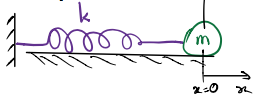
\includegraphics{SpringMass.png}
\caption{Fig. 1: Spring-mass system, again}
\end{figure}

    Now, on top of the force of the spring on the mass, we assume a more
realistic case in which the mass is feeling some friction proportional
to its velocity: \[ F_d = -bv = -b\dot x, \] where the subscript \(d\)
stands for ``damping'', and \(b\) is in kg.s\(^{-1}\). The negative sign
indicates that the force acts on the direction, opposite to that of the
motion, and the proportionality is the simplest mathematical form one
could think of.

\emph{Note: this is a linear approximation again.} \emph{For example,
for a car on a highway (therefore not oscillating, but the force would
have the same expression), the damping force would be proportional to
\(v^2\).} \emph{This would be a lot more difficult to handle,
mathematically speaking.} \emph{And again, this approximation is
sufficient to describe a lot of physical systems.}

    The new equation of motion (EOM) is \begin{equation}
    m \ddot x = -kx - b \dot x \quad \Rightarrow\quad \boxed{\ddot x + \gamma \dot x + \omega_0^2 x = 0,\quad\textrm{with } \gamma = b/m,\ \omega_0^2 = k/m.\ }
    \label{eq:EDO-DSHO}
\end{equation} * \(\gamma\) is often called the \emph{damping factor},
in s\(^{-1}\). * The angular frequency \(\omega_0\) is now called the
\emph{natural (angular) frequency} of the oscillator, i.e., the
frequency of the system if there was no damping. This is a hint that
there could be more than one frequency.

    Before I dig into the math, you should watch the following video of the
two things that can happen when oscillators are damped (that is, a lot
of damping and a little damping), and how the situation that is
in-between, i.e., neither very damped nor weakly damped, is worth
consideration by itself (it is the one that stops first). I will
quantifiy all of my statements later, but before I do, watch the video
so that you at least know what I want to get at.

For those of you who only use the pdf, look up
``\texttt{Critical\ Damping\ -\/-\ xmdemo\ 068}'' in YouTube.

    \begin{Verbatim}[commandchars=\\\{\}]
{\color{incolor}In [{\color{incolor}2}]:} \PY{k+kn}{from} \PY{n+nn}{IPython}\PY{n+nn}{.}\PY{n+nn}{display} \PY{k}{import} \PY{n}{HTML}
        \PY{n}{HTML}\PY{p}{(}\PY{l+s+s1}{\PYZsq{}}\PY{l+s+s1}{\PYZlt{}iframe width=}\PY{l+s+s1}{\PYZdq{}}\PY{l+s+s1}{560}\PY{l+s+s1}{\PYZdq{}}\PY{l+s+s1}{ height=}\PY{l+s+s1}{\PYZdq{}}\PY{l+s+s1}{315}\PY{l+s+s1}{\PYZdq{}}\PY{l+s+s1}{ src=}\PY{l+s+s1}{\PYZdq{}}\PY{l+s+s1}{https://www.youtube.com/embed/99ZE2RGwqSM}\PY{l+s+s1}{\PYZdq{}}\PY{l+s+s1}{ frameborder=}\PY{l+s+s1}{\PYZdq{}}\PY{l+s+s1}{0}\PY{l+s+s1}{\PYZdq{}}\PY{l+s+s1}{ allow=}\PY{l+s+s1}{\PYZdq{}}\PY{l+s+s1}{autoplay; encrypted\PYZhy{}media}\PY{l+s+s1}{\PYZdq{}}\PY{l+s+s1}{ allowfullscreen\PYZgt{}\PYZlt{}/iframe\PYZgt{}}\PY{l+s+s1}{\PYZsq{}}\PY{p}{)}
\end{Verbatim}


\begin{Verbatim}[commandchars=\\\{\}]
{\color{outcolor}Out[{\color{outcolor}2}]:} <IPython.core.display.HTML object>
\end{Verbatim}
            
    \hypertarget{general-solutions}{%
\subsection{General Solutions}\label{general-solutions}}

    The equation above is still a homogeneous second-order ODE: the general
form of the solution will still be the same, and there will be two
coefficients to solve for, for which we will need two initial
conditions.

The form of the solution is slightly more complicated for the DHO than
for the SHO, but we will see that there is a way to make the connection.
For now, let us just \emph{try} a solution:
\[x = a\exp(rt),\quad \textrm{with } (a, r) \in \mathbb C^2.\] ``\(r\)''
stands for \emph{root}: we are looking for the root(s) of the ODE.

Why should \(r\in\mathbb C\)? You will see it in your ODE class, if you
haven't already. As an indication, recall that for
\(\theta \in \mathbb R\), \[\exp(i\theta) = \cos\theta + i\sin\theta.\]
So, if you split the root into its real and imaginary parts, i.e.,
\(rt = r_r t + i\theta t\) with \((r_r, \theta) \in \mathbb R^2\), then
\[\exp(r t) = \left[\cos(\theta t) + i \sin(\theta t)\right]\exp(r_r t).\]
Hopefully, we are starting to see a connection: in the case of
\(r_r < 0\), then the real or imaginary part of \(\exp(r)\) is an
oscillation, multiplying an exponential decay.

We don't know yet if this is the right solution, but let's just say that
it could work.

    Because we want to plug in the trial solution \(a\exp(rt)\) into
eqn.\textasciitilde{}\eqref{eq:EDO-DSHO}, we need the derivatives:
\[ \dot x(t) = ar\exp(rt) = rx(t) \quad\textrm{and}\quad \ddot x = ar^2\exp(rt) = r^2x(t). \]

    We can now plug in:
\[ \ddot x + \gamma \dot x + \omega_0^2 x = r^2 x(t) + \gamma r x(t) + \omega_0^2 x(t) =  0\]
Because we know that \(x(t)\) it is not zero except at specific
instants, and that we need a solution that works at every instant, we
can divide by \(x(t)\): \begin{equation}
    r^2 + \gamma r + \omega_0^2 = 0
\end{equation}

    The equation is a good ol' second-order polynomial, which is solved in
the same way, whether the variable is real or complex. Starting with its
discriminant, which is \begin{equation}
    \Delta = \gamma^2 - 4\omega_0^2.
\end{equation} This quantity will be important later.

    The roots are therefore \begin{equation}
    r_p = -\frac\gamma2 + \sqrt{\frac{\gamma^2}4 -\omega_0^2}\quad \textrm{and}\quad r_m = -\frac\gamma2 - \sqrt{\frac{\gamma^2}4 -\omega_0^2}.
    \label{eq:r_plus_or_minus}
\end{equation} There are two possible roots, and because the ODE is
linear, any linear combination of them is also a solution of the
original equation (\emph{check if you are not sure!}). The most general
solution is therefore \begin{equation}
    x(t) = a_p\exp(r_p t) + a_m\exp(r_mt).
    \label{eq:gensol}
\end{equation}

But careful, the above expression does not work when
\(\omega^2 = \gamma^2/4\), are we are about to see!

    \hypertarget{damping-weak-or-strong}{%
\section{Damping: Weak or Strong?}\label{damping-weak-or-strong}}

    \hypertarget{preliminary-considerations}{%
\subsection{Preliminary
Considerations}\label{preliminary-considerations}}

    Looking at eqn. \eqref{eq:r_plus_or_minus} in detail, we realize that
there are three cases to consider:

\begin{enumerate}
\def\labelenumi{\arabic{enumi}.}
\item
  if \(\gamma^2/4 < \omega_0^2\) (\(\Delta < 0\)), then inside the
  square root is negative, the square root is purely imaginary, and
  \(r_{p,m}\) have a real and an imaginary part. As we are about to see,
  solutions oscillate, on top of decaying exponentially. This case is
  called ``underdamped'', or ``light damping'', because the dissipation
  (\(\gamma\)) is small enough that oscillations (\(\omega_0\)) can
  happen.
\item
  if \(\gamma^2/4 > \omega_0^2\) (\(\Delta >0\)), then inside the square
  root is positive, the square root is real, and both \(r_{p,m}\) are
  real. The solutions are decaying exponentially. This case is called
  ``overdamped'' or ``heavy damping'', because the dissipation
  (\(\gamma\)) is so strong that the oscillation (\(\omega_0\)) cannot
  happen even once.
\item
  if \(\gamma^2/4 = \omega_0^2\) (\(\Delta = 0\)),
  \(r_p = r_m = -\gamma/2\). The solution I wrote at the end of the
  previous section is not even valid anymore, the actual solution being
  \(x(t) = (A + B t)\exp(-\gamma t/2)\), with \(A\) and \(B\) TBD. This
  case is called ``critical damping''
\end{enumerate}

Let us investigate these three cases in more detail.

    \hypertarget{light-damping-omega_02-gamma24}{%
\subsection{\texorpdfstring{Light Damping
(\(\omega_0^2 > \gamma^2/4\))}{Light Damping (\textbackslash{}omega\_0\^{}2 \textgreater{} \textbackslash{}gamma\^{}2/4)}}\label{light-damping-omega_02-gamma24}}

\hypertarget{solution}{%
\subsubsection{Solution}\label{solution}}

Let
\[ \omega_d^2 = \omega_0^2 - \frac{\gamma^2}4 >0 \quad\textrm{and}\quad T_d = \frac{2\pi}{\omega_d}. \]
Therefore,
\[r_{p, m} = -\frac\gamma2 \pm \cplxi\omega_d,\quad \textrm{and} \]
\[ x(t) = \exp\left(- \frac{\gamma t}2\right)\left(a_p\eexp{\cplxi\omega_d t} + a_m\eexp{-\cplxi\omega_d t}\right),\]
with \((a_p, a_m) \in \mathbb C^2\).

    At this point, the problem is more complicated than with the SHO,
because we have four unknown (the real and imaginary parts of \(a_p\)
and \(a_m\)). But we should also have four pieces of information: the
initial position, the initial velocity, and --- and this is going to be
weird --- \emph{the knowledge that \(x\in \mathbb R\)}, and \emph{the
knowledge that \(v\in \mathbb R\)}.

These last two pieces of information help, not so much in
\emph{computing two out of four unknown}, but rather in knowing that
\emph{you only need to compute two unknown}. Indeed, recall that
\(\exp(i\theta) = \cos\theta + i\sin\theta\), as well as the existence
of trigonometric identities such as
\(\cos(a+b) = \cos a \cos b - \sin a \sin b\) (you only need to know hat
they exist). Using a polar decomposition for
\(a_p = |a_p|\exp(i\phi_p)\) and same for \(a_m\), and using all these
identities I just recalled, it is relatively easy to imagine that the
position \(x(t)\) could be re-written in the form of
\[ x(t) = \exp\left(- \frac{\gamma t}2\right)\left(A\cos(\omega_d t + \phi) + i A'\cos(\omega_d t + \phi')\right), \]
with \(A\), \(\phi\), \(A'\) and \(\phi'\) being real numbers, and also
horrible combinations of \(|a_p|\), \(\phi_p\), etc. But then, if we
know that \(x\in \mathbb R\), then \(A' = 0\), and \(\phi'\) becomes
irrelevant. Note that we could do the same thing with \(v\).

So, we now know that those complex exponentials are unnecessarily
complicated, which in fact, what we really need is to solve for
\[ x(t) = A_0\eexp{- \gamma t/2}\cos(\omega_d t +\phi).\]

    \begin{center}\rule{0.5\linewidth}{\linethickness}\end{center}

\emph{Note: Here is a longer explanation, but before I write it, let me
reassure you: I went quicky over it during the lecture, not because it
is so obvious that I don't need to spend some chalk on it, but because
you shouldn't worry about what is essentially a detail.}

So, let us see how we would do if we were to solve the problem with
initial conditions. We would need to define
\(a_p = |a_p|\eexp{i\phi_p}\) and \(a_m = |a_m|\eexp{i\phi_m}\). So far
we have
\[a_p\eexp{\cplxi\omega_d t} + a_m\eexp{-\cplxi\omega_d t} = |a_p|\eexp{\cplxi(\omega_d t +\phi_p)} + |a_m|\eexp{\cplxi(\phi_m - \omega_d t)}\]

Then, remember that \(\eexp{i\theta} = \cos\theta + \cplxi\sin\theta\).
The real part of the expression above is therefore
\[ |a_p|\cos(\omega_d t +\phi_p) + |a_m|\cos(\omega_d t - \phi_m), \]
and its imaginary part is
\[ |a_p|\sin(\omega_d t +\phi_p) - |a_m|\sin(\omega_d t - \phi_m). \]

What a mess, and this is just for the position \(x(t)\): it needs to be
done again for the velocity \(v(t)\).

We now have four unknown (\(|a_p|, |a_m|, \phi_p, \phi_m\)), and four
equations:
\[\textrm{Re}[x(t=0)] = x_0 = \textrm{Re}(a_p + a_m) = |a_p|\cos\phi_p + |a_m|\cos\phi_m, \]
\[\textrm{Im}[x(t=0)] = 0 = \textrm{Im}(a_p + a_m) = |a_p|\sin\phi_p - |a_m|\sin\phi_m, \]
\[\textrm{Re}[v(t=0)] = v_0 = \textrm{Re}(r_p a_p + r_m a_m) = \textrm{something that looks like what is above}, \]
\[\textrm{Im}[v(t=0)] = 0 = \textrm{Im}(r_p a_p + r_m a_m) = \textrm{more of the same but different}. \]

We kept complex numbers around, adding two unknowns, and in response, we
had to add two equations to make sure that the imaginary parts would be
zero.

And then, assuming that we managed to solve the system, what would the
real parts looks like? A bunch of sines and cosines with phases in them,
which we would expand using the formulae
\(\cos(a+b) = \cos a\cos b - \sin a \sin b\) and
\(\sin(a+b) = \sin a\cos b + \cos a \sin b\). The next step would be to
regroup all the \(\sin(\omega_dt)\) together, the \(\cos(\omega_d t)\)
together, and we would find an expression of the type
\[ x_0 = A_1 \cos(\omega_dt) + A_2 \sin(\omega_d t), \] where \(A_1\)
and \(A_2\) would be very long expressions of \(|a_p|\), \(|a_m|\),
\(\phi_p\) and \(\phi_m\). And finally, the expression above can also be
written as \(A\cos(\omega_d t + \phi)\).

The point that I want to make is that a lot of the damage was
self-inflicted: it was completely predictable, based on these
considerations, that the solution was going to take the form
\(A\cos(\omega_dt + \phi)\), and that the imaginary parts were going to
disappear because the solutions had to be real.

Perhaps one last objection you could raise is that King's book starts
directly with \(A \cos(\omega t + \phi)\). Why not do the same? That is
because:

\begin{enumerate}
\def\labelenumi{\arabic{enumi}.}
\tightlist
\item
  at some point, I would need to compute \(v(t) = \dot x(t)\), which
  turns out to be a little complicated if sines and cosines are used;
\item
  this approach allows for a similar treatment between the underdamped
  and overdamped cases (King has to re-boot his derivation, and you lose
  the connection between real and complex exponentials),
\item
  eventually, you should be comfortable with the notion of switching
  from complex exponentials.
\end{enumerate}

\emph{Let me re-iterate though: whether you are now convinced or not,
you will not be tested on such technical points. It will make you a
better engineer and scientist if you understand it, and it will make
your life easier in the classes that come after this one, but you will
not loose points if you don't.}

Back to our regular business.

\begin{center}\rule{0.5\linewidth}{\linethickness}\end{center}

    The velocity is
\[ v(t) = \dot x(t) = A_0\eexp{- \gamma t/2}\left[-\omega_d\sin(\omega_d t + \phi) - \frac{\gamma}{2}\cos(\omega_dt +\phi)\right].\]

    Like in the previous chapter, we have two coefficients to solve for, and
we need two initial conditions to solve it.

\begin{center}\rule{0.5\linewidth}{\linethickness}\end{center}

The specific derivation of \(A_0\) and \(\phi\) that follows doesn't
really matter, and I didn't cover it in class, but I need it for
plotting purposes. Using the initial conditions I used before:

\begin{itemize}
\tightlist
\item
  \(x(t=0) = x_0 = A_0\cos\phi\), and
\item
  \(v(t=0) = 0 = -A_0\left[\omega_d\sin\phi + \frac{\gamma}{2}\cos\phi\right]\ \Rightarrow\ \tan\phi = -\frac\gamma{2\omega_d}\).
\end{itemize}

On the \([0, 2\pi]\) circle, \(\phi\) is the angle for which
\(\cos\phi\) and \(x_0\) have the same sign, because \(A_0>0\) by
definition.

\begin{center}\rule{0.5\linewidth}{\linethickness}\end{center}

    \begin{Verbatim}[commandchars=\\\{\}]
{\color{incolor}In [{\color{incolor}3}]:} \PY{c+c1}{\PYZsh{} let\PYZsq{}s plot}
        \PY{c+c1}{\PYZsh{} This cell is for parameters that I do not intend to change across this chapter.}
        \PY{k+kn}{from} \PY{n+nn}{numpy} \PY{k}{import} \PY{n}{cos}\PY{p}{,} \PY{n}{sin}\PY{p}{,} \PY{n}{exp}\PY{p}{,} \PY{n}{sqrt}\PY{p}{,} \PY{n}{linspace}\PY{p}{,} \PY{n}{pi}\PY{p}{,} \PY{n}{sign}\PY{p}{,} \PY{n}{arctan}
        \PY{k+kn}{import} \PY{n+nn}{matplotlib}\PY{n+nn}{.}\PY{n+nn}{pyplot} \PY{k}{as} \PY{n+nn}{plt}
        \PY{k+kn}{from} \PY{n+nn}{matplotlib} \PY{k}{import} \PY{n}{interactive}
        \PY{n}{interactive}\PY{p}{(}\PY{k+kc}{False}\PY{p}{)}
            
        \PY{n}{x0} \PY{o}{=} \PY{l+m+mf}{4e\PYZhy{}2}  \PY{c+c1}{\PYZsh{} initial position [m]}
        \PY{n}{v0} \PY{o}{=} \PY{l+m+mf}{0.}  \PY{c+c1}{\PYZsh{} initial velocity [m/s]}
        \PY{n}{k} \PY{o}{=} \PY{l+m+mf}{180.}  \PY{c+c1}{\PYZsh{} spring stiffness [N/m]}
        \PY{n}{m} \PY{o}{=} \PY{l+m+mf}{0.8}  \PY{c+c1}{\PYZsh{} mass [kg]}
        \PY{n}{t\PYZus{}end} \PY{o}{=} \PY{l+m+mf}{3.}  \PY{c+c1}{\PYZsh{} final time of plot [s]}
        
        \PY{n}{omega\PYZus{}0} \PY{o}{=} \PY{n}{sqrt}\PY{p}{(}\PY{n}{k}\PY{o}{/}\PY{n}{m}\PY{p}{)}  \PY{c+c1}{\PYZsh{} natural frequency of the oscillation [rad/s]}
        \PY{n}{t} \PY{o}{=} \PY{n}{linspace}\PY{p}{(}\PY{l+m+mf}{0.}\PY{p}{,} \PY{n}{t\PYZus{}end}\PY{p}{,} \PY{l+m+mi}{1024}\PY{p}{)}  \PY{c+c1}{\PYZsh{} time array, from 0 to 0.6 s, 128 points}
        
        \PY{n}{ftsz} \PY{o}{=} \PY{l+m+mi}{13}  \PY{c+c1}{\PYZsh{} font size on plots}
        
        \PY{n}{b\PYZus{}under} \PY{o}{=} \PY{l+m+mf}{1.}  \PY{c+c1}{\PYZsh{} damping [kg/s]}
        
        \PY{c+c1}{\PYZsh{} derived quantities}
        \PY{n}{gamma\PYZus{}under} \PY{o}{=} \PY{n}{b\PYZus{}under}\PY{o}{/}\PY{n}{m}  \PY{c+c1}{\PYZsh{}  damping coefficient [1/s]}
        \PY{n}{omega\PYZus{}d} \PY{o}{=} \PY{n}{sqrt}\PY{p}{(}\PY{n}{omega\PYZus{}0}\PY{o}{*}\PY{o}{*}\PY{l+m+mi}{2} \PY{o}{\PYZhy{}} \PY{n}{gamma\PYZus{}under}\PY{o}{*}\PY{o}{*}\PY{l+m+mi}{2}\PY{o}{/}\PY{l+m+mi}{4}\PY{p}{)}
        \PY{n}{phi} \PY{o}{=} \PY{n}{arctan}\PY{p}{(}\PY{o}{\PYZhy{}}\PY{l+m+mf}{0.5}\PY{o}{*}\PY{n}{gamma\PYZus{}under}\PY{o}{/}\PY{n}{omega\PYZus{}d}\PY{p}{)}
        \PY{k}{if} \PY{n}{sign}\PY{p}{(}\PY{n}{cos}\PY{p}{(}\PY{n}{arctan}\PY{p}{(}\PY{n}{phi}\PY{p}{)}\PY{p}{)}\PY{p}{)} \PY{o}{==} \PY{o}{\PYZhy{}}\PY{n}{sign}\PY{p}{(}\PY{n}{x0}\PY{p}{)}\PY{p}{:}  \PY{c+c1}{\PYZsh{} make sure the correct phase is chosen}
            \PY{n}{phi} \PY{o}{+}\PY{o}{=} \PY{n}{pi}  \PY{c+c1}{\PYZsh{} if not, augment phi by pi to find the other phase}
        \PY{n}{A0} \PY{o}{=} \PY{n}{x0}\PY{o}{/}\PY{n}{cos}\PY{p}{(}\PY{n}{phi}\PY{p}{)}
        
        \PY{n}{T\PYZus{}d} \PY{o}{=} \PY{l+m+mi}{2}\PY{o}{*}\PY{n}{pi}\PY{o}{/}\PY{n}{omega\PYZus{}d}  \PY{c+c1}{\PYZsh{} period of oscillation [s]}
        
        \PY{n}{x\PYZus{}under} \PY{o}{=} \PY{n}{A0}\PY{o}{*}\PY{n}{exp}\PY{p}{(}\PY{o}{\PYZhy{}}\PY{l+m+mf}{0.5}\PY{o}{*}\PY{n}{gamma\PYZus{}under}\PY{o}{*}\PY{n}{t}\PY{p}{)}\PY{o}{*}\PY{n}{cos}\PY{p}{(}\PY{n}{omega\PYZus{}d}\PY{o}{*}\PY{n}{t} \PY{o}{+} \PY{n}{phi}\PY{p}{)}  \PY{c+c1}{\PYZsh{} position [m]}
        \PY{n}{envelope} \PY{o}{=} \PY{n}{A0}\PY{o}{*}\PY{n}{exp}\PY{p}{(}\PY{o}{\PYZhy{}}\PY{l+m+mf}{0.5}\PY{o}{*}\PY{n}{gamma\PYZus{}under}\PY{o}{*}\PY{n}{t}\PY{p}{)}
        
        \PY{n}{fig} \PY{o}{=} \PY{n}{plt}\PY{o}{.}\PY{n}{figure}\PY{p}{(}\PY{p}{)}
        \PY{n}{ax1} \PY{o}{=} \PY{n}{fig}\PY{o}{.}\PY{n}{gca}\PY{p}{(}\PY{p}{)}
        \PY{n}{ax1}\PY{o}{.}\PY{n}{plot}\PY{p}{(}\PY{n}{t}\PY{p}{,} \PY{n}{x\PYZus{}under}\PY{p}{,} \PY{l+s+s1}{\PYZsq{}}\PY{l+s+s1}{b}\PY{l+s+s1}{\PYZsq{}}\PY{p}{,} \PY{n}{label}\PY{o}{=}\PY{l+s+s1}{\PYZsq{}}\PY{l+s+s1}{\PYZdl{}x(t)\PYZdl{}}\PY{l+s+s1}{\PYZsq{}}\PY{p}{)}  \PY{c+c1}{\PYZsh{} plotting the position x}
        \PY{n}{ax1}\PY{o}{.}\PY{n}{plot}\PY{p}{(}\PY{n}{t}\PY{p}{,} \PY{n}{envelope}\PY{p}{,} \PY{l+s+s1}{\PYZsq{}}\PY{l+s+s1}{r\PYZhy{}\PYZhy{}}\PY{l+s+s1}{\PYZsq{}}\PY{p}{,} \PY{n}{label}\PY{o}{=}\PY{l+s+s1}{\PYZsq{}}\PY{l+s+s1}{\PYZdl{}A\PYZus{}0e\PYZca{}}\PY{l+s+s1}{\PYZob{}}\PY{l+s+s1}{\PYZhy{}}\PY{l+s+s1}{\PYZbs{}}\PY{l+s+s1}{gamma t/2\PYZcb{}\PYZdl{}}\PY{l+s+s1}{\PYZsq{}}\PY{p}{)}  \PY{c+c1}{\PYZsh{} plotting the envelope}
        \PY{n}{ax1}\PY{o}{.}\PY{n}{plot}\PY{p}{(}\PY{n}{t}\PY{p}{,} \PY{o}{\PYZhy{}}\PY{n}{envelope}\PY{p}{,} \PY{l+s+s1}{\PYZsq{}}\PY{l+s+s1}{r\PYZhy{}.}\PY{l+s+s1}{\PYZsq{}}\PY{p}{,} \PY{n}{label}\PY{o}{=}\PY{l+s+s1}{\PYZsq{}}\PY{l+s+s1}{\PYZdl{}\PYZhy{}A\PYZus{}0e\PYZca{}}\PY{l+s+s1}{\PYZob{}}\PY{l+s+s1}{\PYZhy{}}\PY{l+s+s1}{\PYZbs{}}\PY{l+s+s1}{gamma t/2\PYZcb{}\PYZdl{}}\PY{l+s+s1}{\PYZsq{}}\PY{p}{)}
        \PY{n}{ax1}\PY{o}{.}\PY{n}{set\PYZus{}xlabel}\PY{p}{(}\PY{l+s+s1}{\PYZsq{}}\PY{l+s+s1}{time [s]}\PY{l+s+s1}{\PYZsq{}}\PY{p}{,} \PY{n}{fontsize}\PY{o}{=}\PY{n}{ftsz}\PY{p}{)} 
        \PY{n}{ax1}\PY{o}{.}\PY{n}{set\PYZus{}ylabel}\PY{p}{(}\PY{l+s+sa}{r}\PY{l+s+s1}{\PYZsq{}}\PY{l+s+s1}{position \PYZdl{}x\PYZdl{} [m]}\PY{l+s+s1}{\PYZsq{}}\PY{p}{,} \PY{n}{fontsize}\PY{o}{=}\PY{n}{ftsz}\PY{p}{)}
        
        \PY{c+c1}{\PYZsh{} annotation to highlight the period}
        \PY{k}{for} \PY{n}{nn} \PY{o+ow}{in} \PY{n+nb}{range}\PY{p}{(}\PY{l+m+mi}{3}\PY{p}{,} \PY{l+m+mi}{5}\PY{p}{)}\PY{p}{:}
            \PY{n}{ax1}\PY{o}{.}\PY{n}{axvline}\PY{p}{(}\PY{n}{nn}\PY{o}{*}\PY{n}{T\PYZus{}d}\PY{p}{,} \PY{n}{color}\PY{o}{=}\PY{l+s+s1}{\PYZsq{}}\PY{l+s+s1}{k}\PY{l+s+s1}{\PYZsq{}}\PY{p}{,} \PY{n}{linestyle}\PY{o}{=}\PY{l+s+s1}{\PYZsq{}}\PY{l+s+s1}{\PYZhy{}.}\PY{l+s+s1}{\PYZsq{}}\PY{p}{)}  \PY{c+c1}{\PYZsh{} the t=nT mark}
        \PY{n}{ax1}\PY{o}{.}\PY{n}{annotate}\PY{p}{(}\PY{n}{s}\PY{o}{=}\PY{l+s+s1}{\PYZsq{}}\PY{l+s+s1}{\PYZsq{}}\PY{p}{,} \PY{n}{xy}\PY{o}{=}\PY{p}{(}\PY{l+m+mi}{3}\PY{o}{*}\PY{n}{T\PYZus{}d}\PY{p}{,} \PY{l+m+mf}{3.5e\PYZhy{}2}\PY{p}{)}\PY{p}{,} \PY{n}{xytext}\PY{o}{=}\PY{p}{(}\PY{l+m+mi}{4}\PY{o}{*}\PY{n}{T\PYZus{}d}\PY{p}{,} \PY{l+m+mf}{3.5e\PYZhy{}2}\PY{p}{)}\PY{p}{,}
                     \PY{n}{arrowprops}\PY{o}{=}\PY{n+nb}{dict}\PY{p}{(}\PY{n}{arrowstyle}\PY{o}{=}\PY{l+s+s1}{\PYZsq{}}\PY{l+s+s1}{\PYZlt{}|\PYZhy{}|\PYZgt{}}\PY{l+s+s1}{\PYZsq{}}\PY{p}{)}\PY{p}{)}  \PY{c+c1}{\PYZsh{} the double arrow}
        \PY{n}{ax1}\PY{o}{.}\PY{n}{text}\PY{p}{(}\PY{l+m+mf}{3.5}\PY{o}{*}\PY{n}{T\PYZus{}d}\PY{p}{,} \PY{l+m+mf}{4.4e\PYZhy{}2}\PY{p}{,} \PY{l+s+sa}{r}\PY{l+s+s1}{\PYZsq{}}\PY{l+s+s1}{\PYZdl{}T\PYZus{}d = 2}\PY{l+s+s1}{\PYZbs{}}\PY{l+s+s1}{pi/}\PY{l+s+s1}{\PYZbs{}}\PY{l+s+s1}{omega\PYZus{}d\PYZdl{}}\PY{l+s+s1}{\PYZsq{}}\PY{p}{,}
                 \PY{n}{verticalalignment}\PY{o}{=}\PY{l+s+s1}{\PYZsq{}}\PY{l+s+s1}{center}\PY{l+s+s1}{\PYZsq{}}\PY{p}{,} \PY{n}{horizontalalignment}\PY{o}{=}\PY{l+s+s1}{\PYZsq{}}\PY{l+s+s1}{center}\PY{l+s+s1}{\PYZsq{}}\PY{p}{,}
                 \PY{n}{backgroundcolor}\PY{o}{=}\PY{l+s+s1}{\PYZsq{}}\PY{l+s+s1}{w}\PY{l+s+s1}{\PYZsq{}}\PY{p}{,} \PY{n}{fontsize}\PY{o}{=}\PY{n}{ftsz}\PY{p}{)}
        
        \PY{c+c1}{\PYZsh{} annotations to highlight the logarithmic decay}
        \PY{n}{ax1}\PY{o}{.}\PY{n}{annotate}\PY{p}{(}\PY{n}{s}\PY{o}{=}\PY{l+s+s1}{\PYZsq{}}\PY{l+s+s1}{\PYZsq{}}\PY{p}{,} \PY{n}{xy}\PY{o}{=}\PY{p}{(}\PY{l+m+mi}{3}\PY{o}{*}\PY{n}{T\PYZus{}d}\PY{p}{,} \PY{l+m+mf}{0.}\PY{p}{)}\PY{p}{,} \PY{n}{xytext}\PY{o}{=}\PY{p}{(}\PY{l+m+mi}{3}\PY{o}{*}\PY{n}{T\PYZus{}d}\PY{p}{,} \PY{n}{A0}\PY{o}{*}\PY{n}{exp}\PY{p}{(}\PY{o}{\PYZhy{}}\PY{l+m+mf}{0.5}\PY{o}{*}\PY{n}{gamma\PYZus{}under}\PY{o}{*}\PY{l+m+mi}{3}\PY{o}{*}\PY{n}{T\PYZus{}d}\PY{p}{)}\PY{p}{)}\PY{p}{,}
                     \PY{n}{arrowprops}\PY{o}{=}\PY{n+nb}{dict}\PY{p}{(}\PY{n}{arrowstyle}\PY{o}{=}\PY{l+s+s1}{\PYZsq{}}\PY{l+s+s1}{\PYZlt{}|\PYZhy{}}\PY{l+s+s1}{\PYZsq{}}\PY{p}{)}\PY{p}{)}  \PY{c+c1}{\PYZsh{} the double arrow}
        \PY{n}{ax1}\PY{o}{.}\PY{n}{text}\PY{p}{(}\PY{l+m+mi}{3}\PY{o}{*}\PY{n}{T\PYZus{}d}\PY{p}{,} \PY{l+m+mf}{1.1}\PY{o}{*}\PY{n}{A0}\PY{o}{*}\PY{n}{exp}\PY{p}{(}\PY{o}{\PYZhy{}}\PY{l+m+mf}{0.5}\PY{o}{*}\PY{n}{gamma\PYZus{}under}\PY{o}{*}\PY{l+m+mi}{3}\PY{o}{*}\PY{n}{T\PYZus{}d}\PY{p}{)}\PY{p}{,} \PY{l+s+s1}{\PYZsq{}}\PY{l+s+s1}{\PYZdl{}A\PYZus{}n\PYZdl{}}\PY{l+s+s1}{\PYZsq{}}\PY{p}{,}
                 \PY{n}{verticalalignment}\PY{o}{=}\PY{l+s+s1}{\PYZsq{}}\PY{l+s+s1}{bottom}\PY{l+s+s1}{\PYZsq{}}\PY{p}{,} \PY{n}{horizontalalignment}\PY{o}{=}\PY{l+s+s1}{\PYZsq{}}\PY{l+s+s1}{left}\PY{l+s+s1}{\PYZsq{}}\PY{p}{,} \PY{n}{fontsize}\PY{o}{=}\PY{n}{ftsz}\PY{p}{)}
        
        \PY{n}{ax1}\PY{o}{.}\PY{n}{annotate}\PY{p}{(}\PY{n}{s}\PY{o}{=}\PY{l+s+s1}{\PYZsq{}}\PY{l+s+s1}{\PYZsq{}}\PY{p}{,} \PY{n}{xy}\PY{o}{=}\PY{p}{(}\PY{l+m+mi}{4}\PY{o}{*}\PY{n}{T\PYZus{}d}\PY{p}{,} \PY{l+m+mf}{0.}\PY{p}{)}\PY{p}{,} \PY{n}{xytext}\PY{o}{=}\PY{p}{(}\PY{l+m+mi}{4}\PY{o}{*}\PY{n}{T\PYZus{}d}\PY{p}{,} \PY{n}{A0}\PY{o}{*}\PY{n}{exp}\PY{p}{(}\PY{o}{\PYZhy{}}\PY{l+m+mf}{0.5}\PY{o}{*}\PY{n}{gamma\PYZus{}under}\PY{o}{*}\PY{l+m+mi}{4}\PY{o}{*}\PY{n}{T\PYZus{}d}\PY{p}{)}\PY{p}{)}\PY{p}{,}
                     \PY{n}{arrowprops}\PY{o}{=}\PY{n+nb}{dict}\PY{p}{(}\PY{n}{arrowstyle}\PY{o}{=}\PY{l+s+s1}{\PYZsq{}}\PY{l+s+s1}{\PYZlt{}|\PYZhy{}}\PY{l+s+s1}{\PYZsq{}}\PY{p}{)}\PY{p}{)}  \PY{c+c1}{\PYZsh{} the double arrow}
        \PY{n}{ax1}\PY{o}{.}\PY{n}{text}\PY{p}{(}\PY{l+m+mi}{4}\PY{o}{*}\PY{n}{T\PYZus{}d}\PY{p}{,} \PY{n}{A0}\PY{o}{*}\PY{n}{exp}\PY{p}{(}\PY{o}{\PYZhy{}}\PY{l+m+mf}{0.5}\PY{o}{*}\PY{n}{gamma\PYZus{}under}\PY{o}{*}\PY{l+m+mi}{4}\PY{o}{*}\PY{n}{T\PYZus{}d}\PY{p}{)}\PY{p}{,} \PY{l+s+s1}{\PYZsq{}}\PY{l+s+s1}{\PYZdl{}A\PYZus{}}\PY{l+s+s1}{\PYZob{}}\PY{l+s+s1}{n+1\PYZcb{}\PYZdl{}}\PY{l+s+s1}{\PYZsq{}}\PY{p}{,}
                 \PY{n}{verticalalignment}\PY{o}{=}\PY{l+s+s1}{\PYZsq{}}\PY{l+s+s1}{bottom}\PY{l+s+s1}{\PYZsq{}}\PY{p}{,} \PY{n}{horizontalalignment}\PY{o}{=}\PY{l+s+s1}{\PYZsq{}}\PY{l+s+s1}{left}\PY{l+s+s1}{\PYZsq{}}\PY{p}{,} \PY{n}{fontsize}\PY{o}{=}\PY{n}{ftsz}\PY{p}{)}
        
        \PY{n}{ax1}\PY{o}{.}\PY{n}{grid}\PY{p}{(}\PY{p}{)}
        \PY{n}{ax1}\PY{o}{.}\PY{n}{axhline}\PY{p}{(}\PY{l+m+mf}{0.}\PY{p}{,} \PY{n}{color}\PY{o}{=}\PY{l+s+s1}{\PYZsq{}}\PY{l+s+s1}{k}\PY{l+s+s1}{\PYZsq{}}\PY{p}{)}  \PY{c+c1}{\PYZsh{} draw the zero\PYZhy{}axis as horizontal line}
        
        \PY{n}{plt}\PY{o}{.}\PY{n}{legend}\PY{p}{(}\PY{p}{)}
        \PY{n}{plt}\PY{o}{.}\PY{n}{savefig}\PY{p}{(}\PY{l+s+s1}{\PYZsq{}}\PY{l+s+s1}{LightlyDampedOscillations.png}\PY{l+s+s1}{\PYZsq{}}\PY{p}{)}
        \PY{n}{plt}\PY{o}{.}\PY{n}{close}\PY{p}{(}\PY{p}{)}
\end{Verbatim}


    \begin{figure}
\centering
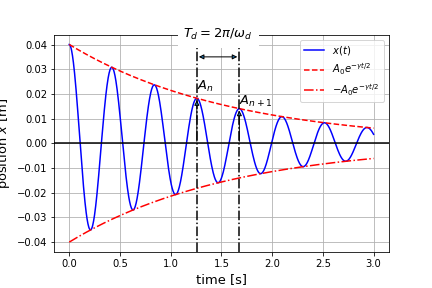
\includegraphics{LightlyDampedOscillations.png}
\caption{Fig. 2: Lightly damped oscillations}
\end{figure}

    The behaviour is that of a (co)sine oscillation of
(\emph{pseudo}-)period \(T_d = 2\pi/\omega_2\) (\emph{not}
\(T_0 = 2\pi/\omega_0\)), like for the SHO, multiplied by an exponential
envelope that makes the waves decay.

\emph{Note: I call \(T_d\) the pseudo-period, King calls it simply the
period. Some of us prefer to refer to periods when systems are perfectly
periodic. Here, the decay breaks the periodicity, and I prefer to talk
about pseudo-periods.}

    A quantity that is often used is the \emph{logarithmic decay} or
\emph{logarithmic decrement}. Let \(A_n = A_0\exp(-\gamma n T_d/2)\) one
local maximum, and \(A_{n+1} = A_0\exp(-\gamma (n+1) T_d/2)\) the next
local maximum, one (pseudo-)period later (see fig. above). Their ratio
is
\[ \frac{A_{n}}{A_{n+1}} = \exp\left(\frac{\gamma T_d}2\right)\textrm{, which does not depend on time nor }n.\]
\[ \Rightarrow \quad \ln\left(\frac{A_{n}}{A_{n+1}}\right) = \frac{\gamma T_d}2\]
The logarithmic decrement is \(\gamma T_d/2\), and the tricky thing is
to remember that the numerator corresponds to the preceding maximum. I
find it confusing because \(A_n/A_{n+1} > 1\) or \(\gamma T_d/2 > 0\),
which is weird for something that decreases. It makes sense because if a
value goes down, the decrement is positive, while the increment would be
negative. It is just a matter of semantics.

    \hypertarget{connection-with-the-sho}{%
\subsubsection{Connection with the SHO}\label{connection-with-the-sho}}

    Now, here is the connection with the SHO problem, because
\(\cos\theta = (\eexp{\cplxi\theta} + \eexp{-\cplxi\theta})/2\) and
\(\sin\theta = (\eexp{\cplxi\theta} - \eexp{-\cplxi\theta})/2\). The
``roots'' of the SHO were simply \(\pm\cplxi\omega t\), with
\(\omega_0 = \omega_d = \omega\). Therefore, it was a particular case of
our current case. Indeed,
\(\tan\phi \propto \gamma =0 \Rightarrow \phi = 0\), implying that
\(A_0 = A = x_0\).

And allow me to drill this one more time: it is still a second-order
ODE, for which we need two initial conditions in order to find a
solution.

    \hypertarget{heavy-damping-omega_02-gamma24}{%
\subsection{\texorpdfstring{Heavy damping
(\(\omega_0^2 < \gamma^2/4\))}{Heavy damping (\textbackslash{}omega\_0\^{}2 \textless{} \textbackslash{}gamma\^{}2/4)}}\label{heavy-damping-omega_02-gamma24}}

    A heavily damped oscillator (\(\Delta = \gamma^2 - 4\omega_0^2 >0\)) is
not even an oscillator: it just crashes down to its initial position
exponentially. If we now define
\[ \alpha = \frac{\sqrt{\Delta}}2 = \sqrt{\frac{\gamma^2}4  - \omega_0^2}\quad\textrm{then} \quad r_{p,m} = -\frac{\gamma}2 \pm \alpha,\]
where I used the notations of eqn.\textasciitilde{}\eqref{eq:gensol}.

The general solution is now
\[ x(t) = a_p \exp\left[\left(\alpha - \frac\gamma2\right)t\right] + a_m \exp\left[-\left(\alpha + \frac\gamma2\right)t\right]. \]
Note that these two exponentials are always decaying, even
\(\exp[(\alpha - \gamma/2)t]\). Indeed,
\[ \alpha^2 = \frac{\gamma^2}4 - \omega_0^2 < \frac{\gamma^2}4 \quad \Rightarrow \quad \alpha < \frac{\gamma} 2\]

    Once again, and for every second-order ODE, we have two coefficients to
solve for, and we need two initial conditions to solve it.

\begin{center}\rule{0.5\linewidth}{\linethickness}\end{center}

And once again, the specific derivation of \(a_p\) and \(a_m\) that
follows doesn't really matter, and I didn't cover it in class, but I
need it for plotting purposes. Using the most general initial
conditions:

\begin{itemize}
\tightlist
\item
  \(x(t=0) = x_0 = a_p + a_m\), and
\item
  \(v(t=0) = v_0 = r_p a_p + r_m a_m\),
\end{itemize}

which is a \(2\times 2\) linear system of equations (the two unknown
being \(a_p\) and \(a_m\)), we find that their solution is
\[a_p = \frac{v_0-r_mx_0}{r_p - r_m}\quad \textrm{and}\quad a_m = \frac{r_px_0 - v_0}{r_p - r_m}. \]

\emph{(Do not memorize these!)}

\begin{center}\rule{0.5\linewidth}{\linethickness}\end{center}

Below, we plot for \(x_0 = 4\) cm and \(v_0 = 0\), just like for the
other examples.

    \begin{Verbatim}[commandchars=\\\{\}]
{\color{incolor}In [{\color{incolor}4}]:} \PY{c+c1}{\PYZsh{} let\PYZsq{}s plot}
        \PY{n}{b\PYZus{}over} \PY{o}{=} \PY{l+m+mf}{1.5}\PY{o}{*}\PY{l+m+mi}{2}\PY{o}{*}\PY{n}{sqrt}\PY{p}{(}\PY{n}{k}\PY{o}{*}\PY{n}{m}\PY{p}{)}  \PY{c+c1}{\PYZsh{} [kg/s]; this makes sure that the discriminant is \PYZgt{}0}
        
        \PY{c+c1}{\PYZsh{} derived quantities}
        \PY{n}{gamma\PYZus{}over} \PY{o}{=} \PY{n}{b\PYZus{}over}\PY{o}{/}\PY{n}{m}  \PY{c+c1}{\PYZsh{}  damping coefficient [1/s]}
        \PY{n}{alpha} \PY{o}{=} \PY{n}{sqrt}\PY{p}{(}\PY{l+m+mf}{0.25}\PY{o}{*}\PY{n}{gamma\PYZus{}over}\PY{o}{*}\PY{o}{*}\PY{l+m+mi}{2} \PY{o}{\PYZhy{}} \PY{n}{omega\PYZus{}0}\PY{o}{*}\PY{o}{*}\PY{l+m+mi}{2}\PY{p}{)}
        \PY{n}{r\PYZus{}p} \PY{o}{=} \PY{n}{alpha} \PY{o}{\PYZhy{}} \PY{l+m+mf}{0.5}\PY{o}{*}\PY{n}{gamma\PYZus{}over}
        \PY{n}{r\PYZus{}m} \PY{o}{=} \PY{o}{\PYZhy{}}\PY{n}{alpha} \PY{o}{\PYZhy{}} \PY{l+m+mf}{0.5}\PY{o}{*}\PY{n}{gamma\PYZus{}over}
        \PY{n}{a\PYZus{}p} \PY{o}{=} \PY{p}{(}\PY{n}{r\PYZus{}m}\PY{o}{*}\PY{n}{x0} \PY{o}{\PYZhy{}} \PY{n}{v0}\PY{p}{)}\PY{o}{/}\PY{p}{(}\PY{n}{r\PYZus{}m} \PY{o}{\PYZhy{}} \PY{n}{r\PYZus{}p}\PY{p}{)}
        \PY{n}{a\PYZus{}m} \PY{o}{=} \PY{p}{(}\PY{n}{v0} \PY{o}{\PYZhy{}} \PY{n}{r\PYZus{}p}\PY{o}{*}\PY{n}{x0}\PY{p}{)}\PY{o}{/}\PY{p}{(}\PY{n}{r\PYZus{}m} \PY{o}{\PYZhy{}} \PY{n}{r\PYZus{}p}\PY{p}{)}
        
        \PY{n}{x\PYZus{}over\PYZus{}p} \PY{o}{=} \PY{n}{a\PYZus{}p}\PY{o}{*}\PY{n}{exp}\PY{p}{(}\PY{n}{r\PYZus{}p}\PY{o}{*}\PY{n}{t}\PY{p}{)}  \PY{c+c1}{\PYZsh{} the first exponential}
        \PY{n}{x\PYZus{}over\PYZus{}m} \PY{o}{=} \PY{n}{a\PYZus{}m}\PY{o}{*}\PY{n}{exp}\PY{p}{(}\PY{n}{r\PYZus{}m}\PY{o}{*}\PY{n}{t}\PY{p}{)}  \PY{c+c1}{\PYZsh{} the second exponential}
        \PY{n}{x\PYZus{}over} \PY{o}{=} \PY{n}{x\PYZus{}over\PYZus{}p} \PY{o}{+} \PY{n}{x\PYZus{}over\PYZus{}m}  \PY{c+c1}{\PYZsh{} position [m]}
        
        \PY{n}{fig} \PY{o}{=} \PY{n}{plt}\PY{o}{.}\PY{n}{figure}\PY{p}{(}\PY{p}{)}
        \PY{n}{ax1} \PY{o}{=} \PY{n}{fig}\PY{o}{.}\PY{n}{gca}\PY{p}{(}\PY{p}{)}
        \PY{n}{ax1}\PY{o}{.}\PY{n}{plot}\PY{p}{(}\PY{n}{t}\PY{p}{,} \PY{n}{x\PYZus{}over\PYZus{}p}\PY{p}{,} \PY{l+s+s1}{\PYZsq{}}\PY{l+s+s1}{r\PYZhy{}\PYZhy{}}\PY{l+s+s1}{\PYZsq{}}\PY{p}{,} \PY{n}{label}\PY{o}{=}\PY{l+s+s1}{\PYZsq{}}\PY{l+s+s1}{\PYZdl{}a\PYZus{}pe\PYZca{}}\PY{l+s+s1}{\PYZob{}}\PY{l+s+s1}{r\PYZus{}p t\PYZcb{}\PYZdl{}}\PY{l+s+s1}{\PYZsq{}}\PY{p}{)}  \PY{c+c1}{\PYZsh{} plotting the 1st exponential}
        \PY{n}{ax1}\PY{o}{.}\PY{n}{plot}\PY{p}{(}\PY{n}{t}\PY{p}{,} \PY{n}{x\PYZus{}over\PYZus{}m}\PY{p}{,} \PY{l+s+s1}{\PYZsq{}}\PY{l+s+s1}{r\PYZhy{}.}\PY{l+s+s1}{\PYZsq{}}\PY{p}{,} \PY{n}{label}\PY{o}{=}\PY{l+s+s1}{\PYZsq{}}\PY{l+s+s1}{\PYZdl{}a\PYZus{}me\PYZca{}}\PY{l+s+s1}{\PYZob{}}\PY{l+s+s1}{r\PYZus{}m t\PYZcb{}\PYZdl{}}\PY{l+s+s1}{\PYZsq{}}\PY{p}{)}  \PY{c+c1}{\PYZsh{} plotting the 2nd exponential}
        \PY{n}{ax1}\PY{o}{.}\PY{n}{plot}\PY{p}{(}\PY{n}{t}\PY{p}{,} \PY{n}{x\PYZus{}over}\PY{p}{,} \PY{l+s+s1}{\PYZsq{}}\PY{l+s+s1}{b}\PY{l+s+s1}{\PYZsq{}}\PY{p}{,} \PY{n}{label}\PY{o}{=}\PY{l+s+s1}{\PYZsq{}}\PY{l+s+s1}{\PYZdl{}x(t)\PYZdl{}}\PY{l+s+s1}{\PYZsq{}}\PY{p}{)}  \PY{c+c1}{\PYZsh{} plotting the position x}
        \PY{n}{ax1}\PY{o}{.}\PY{n}{set\PYZus{}xlabel}\PY{p}{(}\PY{l+s+s1}{\PYZsq{}}\PY{l+s+s1}{time [s]}\PY{l+s+s1}{\PYZsq{}}\PY{p}{,} \PY{n}{fontsize}\PY{o}{=}\PY{n}{ftsz}\PY{p}{)} 
        \PY{n}{ax1}\PY{o}{.}\PY{n}{set\PYZus{}ylabel}\PY{p}{(}\PY{l+s+sa}{r}\PY{l+s+s1}{\PYZsq{}}\PY{l+s+s1}{position \PYZdl{}x\PYZdl{} [m]}\PY{l+s+s1}{\PYZsq{}}\PY{p}{,} \PY{n}{color}\PY{o}{=}\PY{l+s+s1}{\PYZsq{}}\PY{l+s+s1}{b}\PY{l+s+s1}{\PYZsq{}}\PY{p}{,} \PY{n}{fontsize}\PY{o}{=}\PY{n}{ftsz}\PY{p}{)}
        \PY{n}{ax1}\PY{o}{.}\PY{n}{tick\PYZus{}params}\PY{p}{(}\PY{l+s+s1}{\PYZsq{}}\PY{l+s+s1}{y}\PY{l+s+s1}{\PYZsq{}}\PY{p}{,} \PY{n}{colors}\PY{o}{=}\PY{l+s+s1}{\PYZsq{}}\PY{l+s+s1}{b}\PY{l+s+s1}{\PYZsq{}}\PY{p}{)}  \PY{c+c1}{\PYZsh{} color for y\PYZhy{}axis is blue}
        
        \PY{n}{ax1}\PY{o}{.}\PY{n}{grid}\PY{p}{(}\PY{p}{)}
        \PY{n}{ax1}\PY{o}{.}\PY{n}{axhline}\PY{p}{(}\PY{l+m+mf}{0.}\PY{p}{,} \PY{n}{color}\PY{o}{=}\PY{l+s+s1}{\PYZsq{}}\PY{l+s+s1}{k}\PY{l+s+s1}{\PYZsq{}}\PY{p}{)}  \PY{c+c1}{\PYZsh{} draw the zero\PYZhy{}axis as horizontal line}
        
        \PY{n}{plt}\PY{o}{.}\PY{n}{legend}\PY{p}{(}\PY{p}{)}
        \PY{n}{plt}\PY{o}{.}\PY{n}{savefig}\PY{p}{(}\PY{l+s+s1}{\PYZsq{}}\PY{l+s+s1}{StronglyDampedOscillations.png}\PY{l+s+s1}{\PYZsq{}}\PY{p}{)}
        \PY{n}{plt}\PY{o}{.}\PY{n}{close}\PY{p}{(}\PY{p}{)}
\end{Verbatim}


    \begin{figure}
\centering
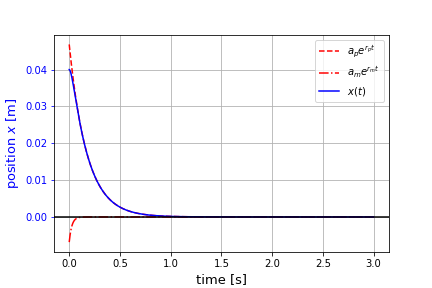
\includegraphics{StronglyDampedOscillations.png}
\caption{Fig. 3: strongly damped ``oscillation''}
\end{figure}

    So, we only have some kind of exponential decay, or more correctly, the
sum of two exponential decays. The most daring of you might try
different initial conditions with the Jupyter notebook (try, e.g.,
\(v_0 > 0\) and \(x_0 = 0\)), but at least, I want you to remember the
general shape of the curve above.

    \hypertarget{critical-damping-omega_02-gamma24}{%
\subsection{\texorpdfstring{Critical damping
(\(\omega_0^2 = \gamma^2/4\))}{Critical damping (\textbackslash{}omega\_0\^{}2 = \textbackslash{}gamma\^{}2/4)}}\label{critical-damping-omega_02-gamma24}}

This case can feel weird: what a coincidence it would be to have both
quantities equal! As a natural scientist, I am actually inclined to
discard it, because yes, coincidences are uninteresting when they occur
naturally. But if I were an engineer, I should not ignore this case:
humans build stuff, and can make this coincidence happen. In the end of
this sub-section, I will show everyday applications. But for now, let's
dive in.

    First of all, eqn.\textasciitilde{}\eqref{eq:gensol} does not work here
with \(a_p\) and \(a_m\) being constant coefficients. Indeed,
\(\omega^2_0 - \gamma^2/2 = 0\) means that \(r_p = r_m = -\gamma/2\).
Therefore, eqn. \eqref{eq:gensol} is written
\[ x(t) = (a_p + a_m)\exp(-\gamma t/2) \] and if \(a_p\) and \(a_m\) are
constant, the velocity is \(v(t) = -\gamma x(t)/2\). This is a problem:
what if we have \(x_0 \neq 0\) and \(v_0 = 0\), like in most of our
previous examples? It is an \emph{overprescribed} or
\emph{overconstrained} problem, in which there is more independent
information than there are degrees of freedom to accommodate it. In
short, it is impossible unless \(x(t) = 0\) at all times, and then, who
cares?

    You might see the reason why in your ODE class, but for now, let's just
accept the fact that in this very particular case, the general solution
is: \[ x(t) = (A + Bt)\exp(-\gamma t / 2), \] which means that the
velocity is
\[v(t) = (B - \gamma A/2 - \gamma Bt/2)\exp(-\gamma t / 2). \] with
\(A\) and \(B\) TBD. Two initial conditions, two unknowns: yay!

    \begin{center}\rule{0.5\linewidth}{\linethickness}\end{center}

And for the last time, I need what follows for plotting purposes. Using
the most general initial conditions:

\begin{itemize}
\tightlist
\item
  \(x(t=0) = x_0 = A\), and
\item
  \(v(t=0) = v_0 = B - \gamma A/2 = B - \gamma x_0/2 \quad\Rightarrow \quad B = v_0 + \gamma x_0/2\).
\end{itemize}

\emph{(Do not learn this!)}

\begin{center}\rule{0.5\linewidth}{\linethickness}\end{center}

Below, we plot for \(x_0 = 4\) cm and \(v_0 = 0\), just like for the
other examples.

    \begin{Verbatim}[commandchars=\\\{\}]
{\color{incolor}In [{\color{incolor}5}]:} \PY{c+c1}{\PYZsh{} let\PYZsq{}s plot}
        \PY{c+c1}{\PYZsh{} I will use the same coefficients except for the damping}
        \PY{n}{b\PYZus{}crit} \PY{o}{=} \PY{l+m+mi}{2}\PY{o}{*}\PY{n}{sqrt}\PY{p}{(}\PY{n}{k}\PY{o}{*}\PY{n}{m}\PY{p}{)}  \PY{c+c1}{\PYZsh{} [kg/s]; this makes sure that the discriminant is 0}
        
        \PY{c+c1}{\PYZsh{} derived quantities}
        \PY{n}{gamma\PYZus{}crit} \PY{o}{=} \PY{n}{b\PYZus{}crit}\PY{o}{/}\PY{n}{m}  \PY{c+c1}{\PYZsh{}  damping coefficient [1/s]}
        \PY{n}{r\PYZus{}c} \PY{o}{=} \PY{o}{\PYZhy{}}\PY{l+m+mf}{0.5}\PY{o}{*}\PY{n}{gamma\PYZus{}crit}
        \PY{n}{A} \PY{o}{=} \PY{n}{x0}
        \PY{n}{B} \PY{o}{=} \PY{n}{v0} \PY{o}{+} \PY{l+m+mf}{0.5}\PY{o}{*}\PY{n}{gamma\PYZus{}crit}\PY{o}{*}\PY{n}{x0}
        
        \PY{n}{x\PYZus{}crit} \PY{o}{=} \PY{p}{(}\PY{n}{A} \PY{o}{+} \PY{n}{B}\PY{o}{*}\PY{n}{t}\PY{p}{)}\PY{o}{*}\PY{n}{exp}\PY{p}{(}\PY{o}{\PYZhy{}}\PY{l+m+mf}{0.5}\PY{o}{*}\PY{n}{gamma\PYZus{}crit}\PY{o}{*}\PY{n}{t}\PY{p}{)}  \PY{c+c1}{\PYZsh{} position [m]}
        
        \PY{n}{fig} \PY{o}{=} \PY{n}{plt}\PY{o}{.}\PY{n}{figure}\PY{p}{(}\PY{p}{)}
        \PY{n}{ax1} \PY{o}{=} \PY{n}{fig}\PY{o}{.}\PY{n}{gca}\PY{p}{(}\PY{p}{)}
        \PY{n}{ax1}\PY{o}{.}\PY{n}{plot}\PY{p}{(}\PY{n}{t}\PY{p}{,} \PY{n}{x\PYZus{}crit}\PY{p}{,} \PY{l+s+s1}{\PYZsq{}}\PY{l+s+s1}{b}\PY{l+s+s1}{\PYZsq{}}\PY{p}{,} \PY{n}{label}\PY{o}{=}\PY{l+s+s1}{\PYZsq{}}\PY{l+s+s1}{\PYZdl{}x(t)\PYZdl{}}\PY{l+s+s1}{\PYZsq{}}\PY{p}{)}  \PY{c+c1}{\PYZsh{} position x}
        \PY{n}{ax1}\PY{o}{.}\PY{n}{set\PYZus{}xlabel}\PY{p}{(}\PY{l+s+s1}{\PYZsq{}}\PY{l+s+s1}{time [s]}\PY{l+s+s1}{\PYZsq{}}\PY{p}{,} \PY{n}{fontsize}\PY{o}{=}\PY{n}{ftsz}\PY{p}{)} 
        \PY{n}{ax1}\PY{o}{.}\PY{n}{set\PYZus{}ylabel}\PY{p}{(}\PY{l+s+sa}{r}\PY{l+s+s1}{\PYZsq{}}\PY{l+s+s1}{position \PYZdl{}x\PYZdl{} [m]}\PY{l+s+s1}{\PYZsq{}}\PY{p}{,} \PY{n}{color}\PY{o}{=}\PY{l+s+s1}{\PYZsq{}}\PY{l+s+s1}{b}\PY{l+s+s1}{\PYZsq{}}\PY{p}{,} \PY{n}{fontsize}\PY{o}{=}\PY{n}{ftsz}\PY{p}{)}
        \PY{n}{ax1}\PY{o}{.}\PY{n}{tick\PYZus{}params}\PY{p}{(}\PY{l+s+s1}{\PYZsq{}}\PY{l+s+s1}{y}\PY{l+s+s1}{\PYZsq{}}\PY{p}{,} \PY{n}{colors}\PY{o}{=}\PY{l+s+s1}{\PYZsq{}}\PY{l+s+s1}{b}\PY{l+s+s1}{\PYZsq{}}\PY{p}{)}  \PY{c+c1}{\PYZsh{} color for y\PYZhy{}axis is blue}
        
        \PY{n}{ax1}\PY{o}{.}\PY{n}{grid}\PY{p}{(}\PY{p}{)}
        \PY{n}{ax1}\PY{o}{.}\PY{n}{axhline}\PY{p}{(}\PY{l+m+mf}{0.}\PY{p}{,} \PY{n}{color}\PY{o}{=}\PY{l+s+s1}{\PYZsq{}}\PY{l+s+s1}{k}\PY{l+s+s1}{\PYZsq{}}\PY{p}{)}  \PY{c+c1}{\PYZsh{} draw the zero\PYZhy{}axis as horizontal line}
        \PY{n}{plt}\PY{o}{.}\PY{n}{savefig}\PY{p}{(}\PY{l+s+s1}{\PYZsq{}}\PY{l+s+s1}{CriticallyDampedOscillations.png}\PY{l+s+s1}{\PYZsq{}}\PY{p}{)}
        \PY{n}{plt}\PY{o}{.}\PY{n}{close}\PY{p}{(}\PY{p}{)}
\end{Verbatim}


    \begin{figure}
\centering
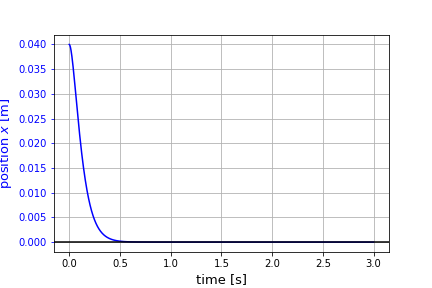
\includegraphics{CriticallyDampedOscillations.png}
\caption{Fig. 4: Critically damped ``oscillation''}
\end{figure}

    Back to the everyday application I promised. Notice how the decay is
faster than the previous, overdamped oscillator. In fact, the
critically-damped oscillator is the one that decays the fastest without
oscillating.

    Indeed, in the overdamped case, there are two exponentials. And because
\(r_m < -\gamma/2\), \(t\eexp{r_m t}\) always decays more slowly that
\(\eexp{-\gamma t/2}\), and the slowest sets the pace (as is hopefully
visible in the figure of the overdamped oscillator above).

Here, \(\alpha = 0\), and so the decay is faster than an overdamped
oscillator.

\emph{Note: more math, but even \(t\eexp{-\beta_1 t}\) decays faster
than \(\eexp{-\beta_2 t}\) if \(\beta_1 > \beta_2 >0\). I do not know at
which point you will learn this calculus result, or if you already did,
but it is true. Just accept this fact for this class.}

    This property can be desirable, a famous example being a car suspension
system, pictured in King's fig. 2.3 (reproduced here).

\begin{figure}
\centering
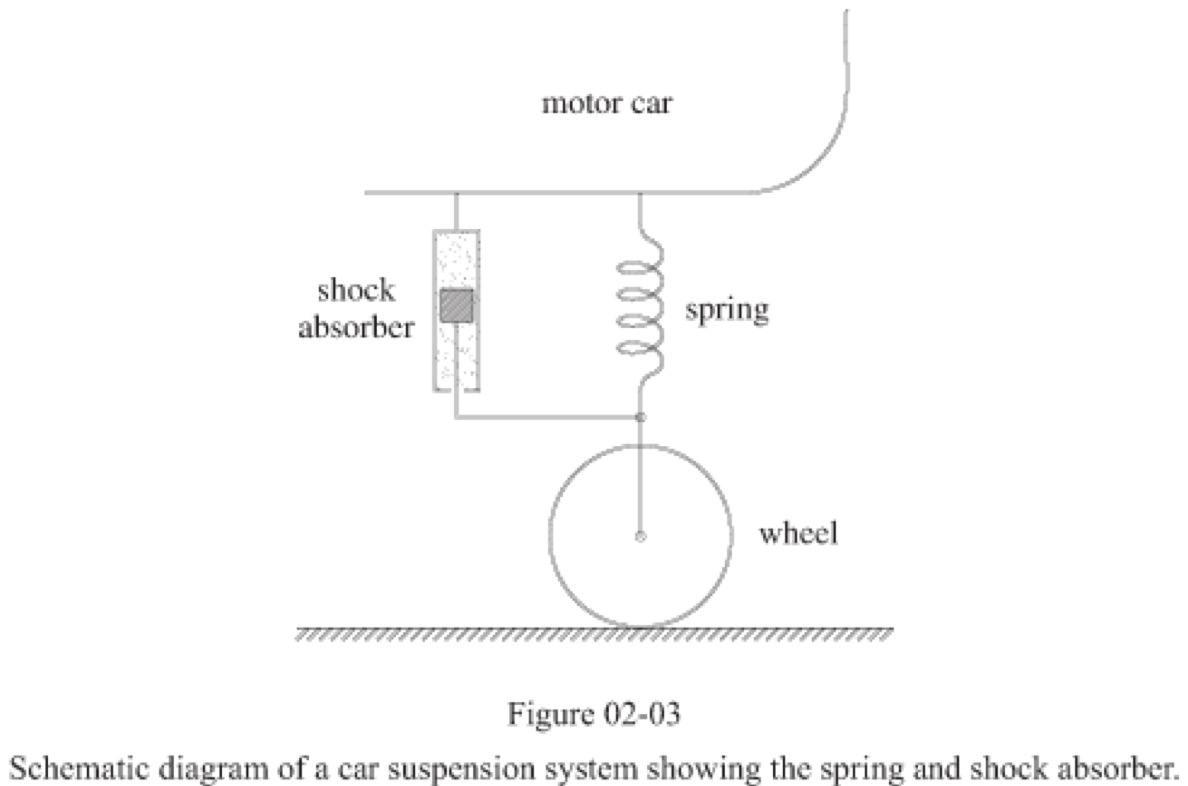
\includegraphics{Suspension.png}
\caption{King 2.3: Suspension}
\end{figure}

    If the spring was too stiff or the shock absorber too soft, shocks would
turn into oscillations and passengers would bounce up and down. On the
other hand, if the spring was not very stiff or the shock absorber too
hard to move, shocks would also be transmitted to the car: the car might
fly a little, fall hard on the ground, and so on. A car maker wants the
shock to be smoothed (not too stiff a spring, not too soft an absorber),
but also that the energy doesn't linger in the car for too long (stiff
enough a spring, soft enough an absorber): it is looking for critical
damping to be achieved for the mass of a car + standard load.

    Other possible applications:

\begin{itemize}
\tightlist
\item
  needle on a meter (don't want to wait for too long for the meter to
  reach value, but don't want it to oscillate around the value either),
\item
  shock absorber + spring for a door that is meant to close
  automatically (don't want the cold winter wind to gush in for too
  long, but don't want the door to slam against the frame either).
\end{itemize}

    \hypertarget{summary}{%
\subsection{Summary}\label{summary}}

I invite you to re-watch the YouTube video I showed towards the
beginning of this chapter, in order to revisit what the three regimes
mean.

I also invite you to play with the tool by following this link:

https://faraday.physics.utoronto.ca/GeneralInterest/Harrison/Flash/ClassMechanics/DampedSHM/DampedSHM.html

Below I plot the three cases that we have seen so far. Note that the
values of all parameters but \(b\) (or \(\gamma\)) are kept constant.
\(b\) (or \(\gamma\)) is the only parameter that we vary across all
cases.

    \begin{Verbatim}[commandchars=\\\{\}]
{\color{incolor}In [{\color{incolor}6}]:} \PY{c+c1}{\PYZsh{} let\PYZsq{}s plot}
        \PY{c+c1}{\PYZsh{} I will use the same parmeters except for the damping}
        \PY{n}{fig} \PY{o}{=} \PY{n}{plt}\PY{o}{.}\PY{n}{figure}\PY{p}{(}\PY{p}{)}
        \PY{n}{ax1} \PY{o}{=} \PY{n}{fig}\PY{o}{.}\PY{n}{gca}\PY{p}{(}\PY{p}{)}
        \PY{n}{ax1}\PY{o}{.}\PY{n}{plot}\PY{p}{(}\PY{n}{t}\PY{p}{,} \PY{n}{x\PYZus{}crit}\PY{p}{,} \PY{l+s+s1}{\PYZsq{}}\PY{l+s+s1}{b}\PY{l+s+s1}{\PYZsq{}}\PY{p}{,} \PY{n}{label}\PY{o}{=}\PY{l+s+s1}{\PYZsq{}}\PY{l+s+s1}{critical}\PY{l+s+s1}{\PYZsq{}}\PY{p}{)}  \PY{c+c1}{\PYZsh{} plotting the position x}
        \PY{n}{ax1}\PY{o}{.}\PY{n}{plot}\PY{p}{(}\PY{n}{t}\PY{p}{,} \PY{n}{x\PYZus{}over}\PY{p}{,} \PY{l+s+s1}{\PYZsq{}}\PY{l+s+s1}{r\PYZhy{}\PYZhy{}}\PY{l+s+s1}{\PYZsq{}}\PY{p}{,} \PY{n}{label}\PY{o}{=}\PY{l+s+s1}{\PYZsq{}}\PY{l+s+s1}{overdamped}\PY{l+s+s1}{\PYZsq{}}\PY{p}{)}  \PY{c+c1}{\PYZsh{} plotting the position x}
        \PY{n}{ax1}\PY{o}{.}\PY{n}{plot}\PY{p}{(}\PY{n}{t}\PY{p}{,} \PY{n}{x\PYZus{}under}\PY{p}{,} \PY{l+s+s1}{\PYZsq{}}\PY{l+s+s1}{g\PYZhy{}.}\PY{l+s+s1}{\PYZsq{}}\PY{p}{,} \PY{n}{label}\PY{o}{=}\PY{l+s+s1}{\PYZsq{}}\PY{l+s+s1}{underdamped}\PY{l+s+s1}{\PYZsq{}}\PY{p}{)}  \PY{c+c1}{\PYZsh{} plotting the position x}
        \PY{n}{ax1}\PY{o}{.}\PY{n}{set\PYZus{}xlabel}\PY{p}{(}\PY{l+s+s1}{\PYZsq{}}\PY{l+s+s1}{time [s]}\PY{l+s+s1}{\PYZsq{}}\PY{p}{,} \PY{n}{fontsize}\PY{o}{=}\PY{n}{ftsz}\PY{p}{)} 
        \PY{n}{ax1}\PY{o}{.}\PY{n}{set\PYZus{}ylabel}\PY{p}{(}\PY{l+s+s1}{\PYZsq{}}\PY{l+s+s1}{position \PYZdl{}x\PYZdl{} [m]}\PY{l+s+s1}{\PYZsq{}}\PY{p}{,} \PY{n}{color}\PY{o}{=}\PY{l+s+s1}{\PYZsq{}}\PY{l+s+s1}{b}\PY{l+s+s1}{\PYZsq{}}\PY{p}{,} \PY{n}{fontsize}\PY{o}{=}\PY{n}{ftsz}\PY{p}{)}
        \PY{n}{ax1}\PY{o}{.}\PY{n}{tick\PYZus{}params}\PY{p}{(}\PY{l+s+s1}{\PYZsq{}}\PY{l+s+s1}{y}\PY{l+s+s1}{\PYZsq{}}\PY{p}{,} \PY{n}{colors}\PY{o}{=}\PY{l+s+s1}{\PYZsq{}}\PY{l+s+s1}{b}\PY{l+s+s1}{\PYZsq{}}\PY{p}{)}  \PY{c+c1}{\PYZsh{} color for y\PYZhy{}axis is blue}
        
        \PY{n}{ax1}\PY{o}{.}\PY{n}{grid}\PY{p}{(}\PY{p}{)}
        \PY{n}{ax1}\PY{o}{.}\PY{n}{axhline}\PY{p}{(}\PY{l+m+mf}{0.}\PY{p}{,} \PY{n}{color}\PY{o}{=}\PY{l+s+s1}{\PYZsq{}}\PY{l+s+s1}{k}\PY{l+s+s1}{\PYZsq{}}\PY{p}{)}  \PY{c+c1}{\PYZsh{} draw the zero\PYZhy{}axis as horizontal line}
        
        \PY{n}{plt}\PY{o}{.}\PY{n}{legend}\PY{p}{(}\PY{p}{)}
        \PY{n}{plt}\PY{o}{.}\PY{n}{savefig}\PY{p}{(}\PY{l+s+s1}{\PYZsq{}}\PY{l+s+s1}{DampedOscillations.png}\PY{l+s+s1}{\PYZsq{}}\PY{p}{)}
        \PY{n}{plt}\PY{o}{.}\PY{n}{close}\PY{p}{(}\PY{p}{)}
\end{Verbatim}


    \begin{Verbatim}[commandchars=\\\{\}]
{\color{incolor}In [{\color{incolor}7}]:} \PY{o}{!}\PY{o}{[}Fig. \PY{l+m}{5}: Damped oscillations, a summary\PY{o}{]}\PY{o}{(}DampedOscillations.png\PY{o}{)}
\end{Verbatim}


    \begin{Verbatim}[commandchars=\\\{\}]
/bin/sh: 1: Syntax error: "(" unexpected

    \end{Verbatim}

    Note above how the transition from under- to overdamped happens, and how
an overdamped oscillator takes too long to land.

    \begin{enumerate}
\def\labelenumi{\arabic{enumi}.}
\item
  \(\gamma^2/4 < \omega_0^2\): light damping, or underdamped oscillator.
  Damped oscillations.
\item
  \(\gamma^2/4 > \omega_0^2\): heavy damping, or overdamped oscillator.
  Exponential decay to equilibrium position.
\item
  \(\gamma^2/4 = \omega_0^2\): critical damping. Quickest return to
  equilibrium position without overshoot.
\end{enumerate}

    \hypertarget{energy}{%
\section{Energy}\label{energy}}

\hypertarget{general-considerations}{%
\subsection{General Considerations}\label{general-considerations}}

Whether the mass moves or is held in place, the friction does not
represent an energy reservoir like KE or PE do: it merely removes
mechanical energy from the system. Therefore, the energy of the system
has the same expression: \[ E = K + U = \frac12 m v^2 + \frac12 kx^2.\]

    What the existence of friction/damping change is the \emph{time
evolution} of the mechanical energy: it decays. Note that I am not
violating the conservation of total energy of a closed system. This is
because damping allows to exchange energy with other types of energy
reservoirs. For example, friction can create heat. The energy is still
present in the system, but it is in the form of \emph{internal energy},
not mechanical energy. The energy could also be exchanged with the
outside, for example in the form of vibrations (mechanical vibrations or
sound waves). But in any case, the \emph{total energy of the closed
system}, which may include the entire universe if need be, stays
constant.

In the SHO, \(E\) was constant because without any damping, the SHO is
effectively a closed system, a system that cannot exchange energy with
other reservoirs of energy, be they internal or external.

    The damping does not represent an energy reservoir, but is does
represent a leak, or a drain, of energy:

\[ \ode{E}t = \ode{}{t}\left(\frac12 m v^2 +\frac12k x^2\right) = mv\dot v + kx\dot x = (ma + kx)v, \]
and because \(ma = -kx - bv\), \[ \boxed{\ode{E}t =  -bv^2}. \] The
mechanical energy loss is directly attributable to the damping. Notice
how the damping rate depends on the \emph{square} of the linear
quantities, here, \(v^2\). This is a reminder of the quadratic
dependence of energy quantities versus linear quantities (``double the
amplitude, quadruple the energy'').

    \hypertarget{underdamped-harmonic-oscillator-omega_02-gamma24}{%
\subsection{\texorpdfstring{Underdamped Harmonic Oscillator
(\(\omega_0^2 > \gamma^2/4\))}{Underdamped Harmonic Oscillator (\textbackslash{}omega\_0\^{}2 \textgreater{} \textbackslash{}gamma\^{}2/4)}}\label{underdamped-harmonic-oscillator-omega_02-gamma24}}

The potential energy is
\[ U = \frac12 k x^2 =  \frac12 k A_0^2 \cos^2(\omega_d t + \phi) \eexp{-\gamma t}  \]

    The kinetic energy is \begin{align*}
    K & = \frac12 m A_0^2 \eexp{- \gamma t}\left[-\omega_d\sin(\omega_d t + \phi) - \frac{\gamma}{2}\cos(\omega_dt +\phi)\right]^2 \\
      & = \frac12 m A_0^2 \omega_d^2 \eexp{- \gamma t}\left[\sin(\omega_d t + \phi) + \frac{\gamma}{2\omega_d}\cos(\omega_dt +\phi)\right]^2 \\
      & \approx \frac12 m A_0^2 \omega_0^2 \eexp{- \gamma t}\sin^2(\omega_d t + \phi),
\end{align*} where the last bit of approximation is valid when
\(\omega_0 \gg \gamma/2 \Rightarrow \gamma/(2\omega_d) \approx \gamma/(2\omega_0) \ll 1\).

    The mechanical energy is therefore (under the
\(\gamma/(2\omega_0) \ll 1\), \(\omega_d \approx \omega_0\)
approximation):
\[ E = K + U \approx \frac12 A_0^2 \eexp{- \gamma t}\left[m\omega_0^2 \sin^2(\omega_d t + \phi) + k \cos^2(\omega_d t + \phi)\right], \]
\[\textrm{Recall that } m\omega_0^2 = k \textrm{ and } \cos^2 + \sin^2 = 1\quad \Rightarrow\quad \boxed{E = \frac12 k A_0^2 \eexp{- \gamma t}}.\]

    The point to remember is that \textbf{for a lightly damped oscillator,
the mechanical energy decays exponentially.} The e-folding decay time
scale \(1/\gamma\) is also called the \emph{lifetime} of the
oscillation.

    \emph{Remarks:}

\begin{itemize}
\tightlist
\item
  \emph{We only ask you to remember this \(\gamma/(2\omega_0) \ll 1\)
  limiting behaviour. Below, I plot the unapproximated version of \(K\)
  and \(E\) for your information, not because you have to remember it.}
\item
  \emph{Above, I made a few approximations in a row, which can be
  dangerous business if we are not careful. The proper way to do it
  would be to define \(\varepsilon = \gamma/(2\omega_0)\), to
  Taylor-expand each term, and to collect all the leading-order terms.
  Such mathematical refinery is a bit too technical for what is required
  of you in this class.}
\end{itemize}

    \begin{Verbatim}[commandchars=\\\{\}]
{\color{incolor}In [{\color{incolor}8}]:} \PY{c+c1}{\PYZsh{} let\PYZsq{}s plot, with the previous numerical values for the underdamped oscillator}
        \PY{n}{v\PYZus{}under} \PY{o}{=} \PY{n}{A0}\PY{o}{*}\PY{n}{exp}\PY{p}{(}\PY{o}{\PYZhy{}}\PY{l+m+mf}{0.5}\PY{o}{*}\PY{n}{gamma\PYZus{}under}\PY{o}{*}\PY{n}{t}\PY{p}{)}\PY{o}{*}\PY{p}{(}\PY{o}{\PYZhy{}}\PY{n}{omega\PYZus{}d}\PY{o}{*}\PY{n}{sin}\PY{p}{(}\PY{n}{omega\PYZus{}d}\PY{o}{*}\PY{n}{t} \PY{o}{+} \PY{n}{phi}\PY{p}{)}
                                              \PY{o}{\PYZhy{}} \PY{l+m+mf}{0.5}\PY{o}{*}\PY{n}{gamma\PYZus{}under}\PY{o}{*}\PY{n}{cos}\PY{p}{(}\PY{n}{omega\PYZus{}d}\PY{o}{*}\PY{n}{t} \PY{o}{+} \PY{n}{phi}\PY{p}{)}\PY{p}{)}
        \PY{n}{v\PYZus{}under\PYZus{}approx} \PY{o}{=} \PY{o}{\PYZhy{}}\PY{n}{A0}\PY{o}{*}\PY{n}{exp}\PY{p}{(}\PY{o}{\PYZhy{}}\PY{l+m+mf}{0.5}\PY{o}{*}\PY{n}{gamma\PYZus{}under}\PY{o}{*}\PY{n}{t}\PY{p}{)}\PY{o}{*}\PY{n}{omega\PYZus{}0}\PY{o}{*}\PY{n}{sin}\PY{p}{(}\PY{n}{omega\PYZus{}d}\PY{o}{*}\PY{n}{t} \PY{o}{+} \PY{n}{phi}\PY{p}{)}
        
        \PY{n}{K\PYZus{}under} \PY{o}{=} \PY{l+m+mf}{0.5}\PY{o}{*}\PY{n}{m}\PY{o}{*}\PY{n}{v\PYZus{}under}\PY{o}{*}\PY{o}{*}\PY{l+m+mi}{2}
        \PY{n}{K\PYZus{}under\PYZus{}approx} \PY{o}{=} \PY{l+m+mf}{0.5}\PY{o}{*}\PY{n}{m}\PY{o}{*}\PY{n}{v\PYZus{}under\PYZus{}approx}\PY{o}{*}\PY{o}{*}\PY{l+m+mi}{2}
        
        \PY{n}{U\PYZus{}under} \PY{o}{=} \PY{l+m+mf}{0.5}\PY{o}{*}\PY{n}{k}\PY{o}{*}\PY{n}{x\PYZus{}under}\PY{o}{*}\PY{o}{*}\PY{l+m+mi}{2}
        
        \PY{n}{E\PYZus{}under} \PY{o}{=} \PY{n}{K\PYZus{}under} \PY{o}{+} \PY{n}{U\PYZus{}under}
        \PY{n}{E\PYZus{}under\PYZus{}approx} \PY{o}{=} \PY{n}{K\PYZus{}under\PYZus{}approx} \PY{o}{+} \PY{n}{U\PYZus{}under}
        
        \PY{n}{fig} \PY{o}{=} \PY{n}{plt}\PY{o}{.}\PY{n}{figure}\PY{p}{(}\PY{p}{)}
        \PY{n}{ax1} \PY{o}{=} \PY{n}{fig}\PY{o}{.}\PY{n}{gca}\PY{p}{(}\PY{p}{)}
        \PY{n}{ax1}\PY{o}{.}\PY{n}{plot}\PY{p}{(}\PY{n}{t}\PY{p}{,} \PY{n}{K\PYZus{}under}\PY{p}{,} \PY{l+s+s1}{\PYZsq{}}\PY{l+s+s1}{b\PYZhy{}.}\PY{l+s+s1}{\PYZsq{}}\PY{p}{,} \PY{n}{label}\PY{o}{=}\PY{l+s+s1}{\PYZsq{}}\PY{l+s+s1}{\PYZdl{}K(t)\PYZdl{}}\PY{l+s+s1}{\PYZsq{}}\PY{p}{)}  \PY{c+c1}{\PYZsh{} unapproximated kinetic energy}
        \PY{n}{ax1}\PY{o}{.}\PY{n}{plot}\PY{p}{(}\PY{n}{t}\PY{p}{,} \PY{n}{K\PYZus{}under\PYZus{}approx}\PY{p}{,} \PY{l+s+s1}{\PYZsq{}}\PY{l+s+s1}{b}\PY{l+s+s1}{\PYZsq{}}\PY{p}{,} \PY{n}{label}\PY{o}{=}\PY{l+s+s1}{\PYZsq{}}\PY{l+s+s1}{\PYZdl{}K(t)\PYZdl{}, approx.}\PY{l+s+s1}{\PYZsq{}}\PY{p}{)}  \PY{c+c1}{\PYZsh{} approximated kinetic energy}
        \PY{n}{ax1}\PY{o}{.}\PY{n}{plot}\PY{p}{(}\PY{n}{t}\PY{p}{,} \PY{n}{U\PYZus{}under}\PY{p}{,} \PY{l+s+s1}{\PYZsq{}}\PY{l+s+s1}{g\PYZhy{}\PYZhy{}}\PY{l+s+s1}{\PYZsq{}}\PY{p}{,} \PY{n}{label}\PY{o}{=}\PY{l+s+s1}{\PYZsq{}}\PY{l+s+s1}{\PYZdl{}U(t)\PYZdl{}}\PY{l+s+s1}{\PYZsq{}}\PY{p}{)}  \PY{c+c1}{\PYZsh{} potential energy}
        \PY{n}{ax1}\PY{o}{.}\PY{n}{plot}\PY{p}{(}\PY{n}{t}\PY{p}{,} \PY{n}{E\PYZus{}under}\PY{p}{,} \PY{l+s+s1}{\PYZsq{}}\PY{l+s+s1}{r\PYZhy{}.}\PY{l+s+s1}{\PYZsq{}}\PY{p}{,} \PY{n}{label}\PY{o}{=}\PY{l+s+s1}{\PYZsq{}}\PY{l+s+s1}{\PYZdl{}E(t)\PYZdl{}}\PY{l+s+s1}{\PYZsq{}}\PY{p}{)}  \PY{c+c1}{\PYZsh{} unapproximated mechanical energy}
        \PY{n}{ax1}\PY{o}{.}\PY{n}{plot}\PY{p}{(}\PY{n}{t}\PY{p}{,} \PY{n}{E\PYZus{}under\PYZus{}approx}\PY{p}{,} \PY{l+s+s1}{\PYZsq{}}\PY{l+s+s1}{r}\PY{l+s+s1}{\PYZsq{}}\PY{p}{,} \PY{n}{label}\PY{o}{=}\PY{l+s+s1}{\PYZsq{}}\PY{l+s+s1}{\PYZdl{}E(t)\PYZdl{}, approx.}\PY{l+s+s1}{\PYZsq{}}\PY{p}{)}  \PY{c+c1}{\PYZsh{} approximated mechanical energy}
        \PY{n}{ax1}\PY{o}{.}\PY{n}{set\PYZus{}xlabel}\PY{p}{(}\PY{l+s+s1}{\PYZsq{}}\PY{l+s+s1}{time [s]}\PY{l+s+s1}{\PYZsq{}}\PY{p}{,} \PY{n}{fontsize}\PY{o}{=}\PY{n}{ftsz}\PY{p}{)} 
        \PY{n}{ax1}\PY{o}{.}\PY{n}{set\PYZus{}ylabel}\PY{p}{(}\PY{l+s+s1}{\PYZsq{}}\PY{l+s+s1}{Energies [J]}\PY{l+s+s1}{\PYZsq{}}\PY{p}{,} \PY{n}{fontsize}\PY{o}{=}\PY{n}{ftsz}\PY{p}{)}
        
        \PY{n}{ax1}\PY{o}{.}\PY{n}{grid}\PY{p}{(}\PY{p}{)}
        \PY{n}{ax1}\PY{o}{.}\PY{n}{axhline}\PY{p}{(}\PY{l+m+mf}{0.}\PY{p}{,} \PY{n}{color}\PY{o}{=}\PY{l+s+s1}{\PYZsq{}}\PY{l+s+s1}{k}\PY{l+s+s1}{\PYZsq{}}\PY{p}{)}  \PY{c+c1}{\PYZsh{} draw the zero\PYZhy{}axis as horizontal line}
        
        \PY{n}{plt}\PY{o}{.}\PY{n}{legend}\PY{p}{(}\PY{p}{)}
        \PY{n}{plt}\PY{o}{.}\PY{n}{savefig}\PY{p}{(}\PY{l+s+s1}{\PYZsq{}}\PY{l+s+s1}{LightlyDampedEnergy.png}\PY{l+s+s1}{\PYZsq{}}\PY{p}{)}
        \PY{n}{plt}\PY{o}{.}\PY{n}{close}\PY{p}{(}\PY{p}{)}
\end{Verbatim}


    \begin{figure}
\centering
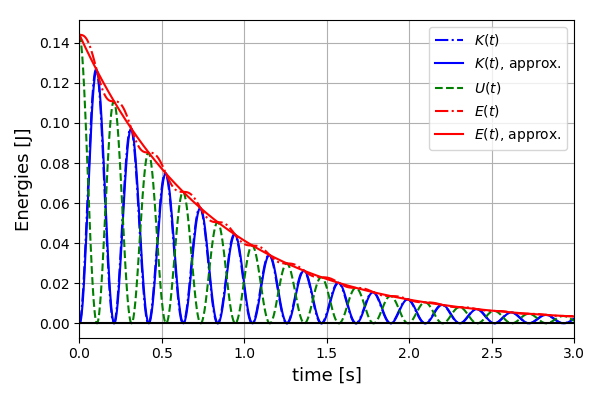
\includegraphics{LightlyDampedEnergy.png}
\caption{Fig. 5: Energy of lightly damped oscillations}
\end{figure}

    \begin{Verbatim}[commandchars=\\\{\}]
{\color{incolor}In [{\color{incolor}9}]:} \PY{n+nb}{print}\PY{p}{(}\PY{l+s+s1}{\PYZsq{}}\PY{l+s+s1}{gamma/(2*omega0) = }\PY{l+s+si}{\PYZob{}0:.1e\PYZcb{}}\PY{l+s+s1}{\PYZsq{}}\PY{o}{.}\PY{n}{format}\PY{p}{(}\PY{l+m+mf}{0.5}\PY{o}{*}\PY{n}{gamma\PYZus{}under}\PY{o}{/}\PY{n}{omega\PYZus{}0}\PY{p}{)}\PY{p}{)}
        \PY{n+nb}{print}\PY{p}{(}\PY{l+s+s1}{\PYZsq{}}\PY{l+s+s1}{Q = }\PY{l+s+si}{\PYZob{}0:.1e\PYZcb{}}\PY{l+s+s1}{\PYZsq{}}\PY{o}{.}\PY{n}{format}\PY{p}{(}\PY{n}{omega\PYZus{}0}\PY{o}{/}\PY{n}{gamma\PYZus{}under}\PY{p}{)}\PY{p}{)}
        \PY{n+nb}{print}\PY{p}{(}\PY{l+s+s1}{\PYZsq{}}\PY{l+s+s1}{1/gamma = }\PY{l+s+si}{\PYZob{}0:.1e\PYZcb{}}\PY{l+s+s1}{ s}\PY{l+s+s1}{\PYZsq{}}\PY{o}{.}\PY{n}{format}\PY{p}{(}\PY{n}{gamma\PYZus{}under}\PY{o}{*}\PY{o}{*}\PY{o}{\PYZhy{}}\PY{l+m+mi}{1}\PY{p}{)}\PY{p}{)}
\end{Verbatim}


    \begin{Verbatim}[commandchars=\\\{\}]
gamma/(2*omega0) = 4.2e-02
Q = 1.2e+01
1/gamma = 8.0e-01 s

    \end{Verbatim}

    As you can see above, it is hard to distinguish the curves with or
without the \(\gamma/(2\omega) \ll 1\) approximation, meaning that even
for an e-folding decay scale of a few pseudo-oscillation periods (here,
\(\gamma/(2\omega) \approx 0.042\)), the approximation is a good one.

    \hypertarget{over--and-critically-damped-oscillators}{%
\subsection{Over- and Critically damped
oscillators}\label{over--and-critically-damped-oscillators}}

    There isn't much to say about these cases: their energy just decays, and
because of the quadratic dependence of the energy on the amplitude, they
decay twice as fast as the envelope of the oscillations.

I will just plot all three cases in one plot.

    \begin{Verbatim}[commandchars=\\\{\}]
{\color{incolor}In [{\color{incolor}10}]:} \PY{c+c1}{\PYZsh{} let\PYZsq{}s plot, with the previous numerical values fir the underdamped oscillator}
         \PY{c+c1}{\PYZsh{} Energies for the critical case}
         \PY{n}{v\PYZus{}crit} \PY{o}{=} \PY{p}{(}\PY{n}{B} \PY{o}{\PYZhy{}} \PY{l+m+mf}{0.5}\PY{o}{*}\PY{n}{gamma\PYZus{}crit}\PY{o}{*}\PY{n}{A} \PY{o}{\PYZhy{}} \PY{l+m+mf}{0.5}\PY{o}{*}\PY{n}{gamma\PYZus{}crit}\PY{o}{*}\PY{n}{B}\PY{o}{*}\PY{n}{t}\PY{p}{)}\PY{o}{*}\PY{n}{exp}\PY{p}{(}\PY{o}{\PYZhy{}}\PY{l+m+mf}{0.5}\PY{o}{*}\PY{n}{gamma\PYZus{}crit}\PY{o}{*}\PY{n}{t}\PY{p}{)}
         \PY{c+c1}{\PYZsh{} above: velocity in critical case}
         \PY{n}{K\PYZus{}crit} \PY{o}{=} \PY{l+m+mf}{0.5}\PY{o}{*}\PY{n}{m}\PY{o}{*}\PY{n}{v\PYZus{}crit}\PY{o}{*}\PY{o}{*}\PY{l+m+mi}{2}  \PY{c+c1}{\PYZsh{} kinetic}
         \PY{n}{U\PYZus{}crit} \PY{o}{=} \PY{l+m+mf}{0.5}\PY{o}{*}\PY{n}{k}\PY{o}{*}\PY{n}{x\PYZus{}crit}\PY{o}{*}\PY{o}{*}\PY{l+m+mi}{2}  \PY{c+c1}{\PYZsh{} potential}
         \PY{n}{E\PYZus{}crit} \PY{o}{=} \PY{n}{K\PYZus{}crit} \PY{o}{+} \PY{n}{U\PYZus{}crit}  \PY{c+c1}{\PYZsh{} mechanical}
         
         \PY{c+c1}{\PYZsh{} Energies for the overdamped case}
         \PY{n}{v\PYZus{}over\PYZus{}p} \PY{o}{=} \PY{n}{r\PYZus{}p}\PY{o}{*}\PY{n}{a\PYZus{}p}\PY{o}{*}\PY{n}{exp}\PY{p}{(}\PY{n}{r\PYZus{}p}\PY{o}{*}\PY{n}{t}\PY{p}{)}  \PY{c+c1}{\PYZsh{} velocity of the first exponential}
         \PY{n}{v\PYZus{}over\PYZus{}m} \PY{o}{=} \PY{n}{r\PYZus{}m}\PY{o}{*}\PY{n}{a\PYZus{}m}\PY{o}{*}\PY{n}{exp}\PY{p}{(}\PY{n}{r\PYZus{}m}\PY{o}{*}\PY{n}{t}\PY{p}{)}  \PY{c+c1}{\PYZsh{} velocity of the second exponential}
         \PY{n}{v\PYZus{}over} \PY{o}{=} \PY{n}{v\PYZus{}over\PYZus{}p} \PY{o}{+} \PY{n}{v\PYZus{}over\PYZus{}m}  \PY{c+c1}{\PYZsh{} veloctiy in the overdamped case [m/s]}
         \PY{n}{K\PYZus{}over} \PY{o}{=} \PY{l+m+mf}{0.5}\PY{o}{*}\PY{n}{m}\PY{o}{*}\PY{n}{v\PYZus{}over}\PY{o}{*}\PY{o}{*}\PY{l+m+mi}{2}  \PY{c+c1}{\PYZsh{} kinetic}
         \PY{n}{U\PYZus{}over} \PY{o}{=} \PY{l+m+mf}{0.5}\PY{o}{*}\PY{n}{k}\PY{o}{*}\PY{n}{x\PYZus{}over}\PY{o}{*}\PY{o}{*}\PY{l+m+mi}{2}  \PY{c+c1}{\PYZsh{} potential}
         \PY{n}{E\PYZus{}over} \PY{o}{=} \PY{n}{K\PYZus{}over} \PY{o}{+} \PY{n}{U\PYZus{}over}  \PY{c+c1}{\PYZsh{} mechanical}
         
         \PY{c+c1}{\PYZsh{} plot}
         \PY{n}{fig} \PY{o}{=} \PY{n}{plt}\PY{o}{.}\PY{n}{figure}\PY{p}{(}\PY{p}{)}
         \PY{n}{ax1} \PY{o}{=} \PY{n}{fig}\PY{o}{.}\PY{n}{gca}\PY{p}{(}\PY{p}{)}
         \PY{n}{ax1}\PY{o}{.}\PY{n}{plot}\PY{p}{(}\PY{n}{t}\PY{p}{,} \PY{n}{E\PYZus{}under\PYZus{}approx}\PY{p}{,} \PY{l+s+s1}{\PYZsq{}}\PY{l+s+s1}{g\PYZhy{}.}\PY{l+s+s1}{\PYZsq{}}\PY{p}{,} \PY{n}{label}\PY{o}{=}\PY{l+s+s1}{\PYZsq{}}\PY{l+s+s1}{underdamped, approx.}\PY{l+s+s1}{\PYZsq{}}\PY{p}{)}
         \PY{n}{ax1}\PY{o}{.}\PY{n}{plot}\PY{p}{(}\PY{n}{t}\PY{p}{,} \PY{n}{E\PYZus{}over}\PY{p}{,} \PY{l+s+s1}{\PYZsq{}}\PY{l+s+s1}{r\PYZhy{}\PYZhy{}}\PY{l+s+s1}{\PYZsq{}}\PY{p}{,} \PY{n}{label}\PY{o}{=}\PY{l+s+s1}{\PYZsq{}}\PY{l+s+s1}{overdamped}\PY{l+s+s1}{\PYZsq{}}\PY{p}{)}
         \PY{n}{ax1}\PY{o}{.}\PY{n}{plot}\PY{p}{(}\PY{n}{t}\PY{p}{,} \PY{n}{E\PYZus{}crit}\PY{p}{,} \PY{l+s+s1}{\PYZsq{}}\PY{l+s+s1}{b}\PY{l+s+s1}{\PYZsq{}}\PY{p}{,} \PY{n}{label}\PY{o}{=}\PY{l+s+s1}{\PYZsq{}}\PY{l+s+s1}{critical}\PY{l+s+s1}{\PYZsq{}}\PY{p}{)}
         \PY{n}{ax1}\PY{o}{.}\PY{n}{set\PYZus{}xlabel}\PY{p}{(}\PY{l+s+s1}{\PYZsq{}}\PY{l+s+s1}{time [s]}\PY{l+s+s1}{\PYZsq{}}\PY{p}{,} \PY{n}{fontsize}\PY{o}{=}\PY{n}{ftsz}\PY{p}{)} 
         \PY{n}{ax1}\PY{o}{.}\PY{n}{set\PYZus{}ylabel}\PY{p}{(}\PY{l+s+s1}{\PYZsq{}}\PY{l+s+s1}{Energies [J]}\PY{l+s+s1}{\PYZsq{}}\PY{p}{,} \PY{n}{fontsize}\PY{o}{=}\PY{n}{ftsz}\PY{p}{)}
         
         \PY{n}{ax1}\PY{o}{.}\PY{n}{grid}\PY{p}{(}\PY{p}{)}
         \PY{n}{ax1}\PY{o}{.}\PY{n}{axhline}\PY{p}{(}\PY{l+m+mf}{0.}\PY{p}{,} \PY{n}{color}\PY{o}{=}\PY{l+s+s1}{\PYZsq{}}\PY{l+s+s1}{k}\PY{l+s+s1}{\PYZsq{}}\PY{p}{)}  \PY{c+c1}{\PYZsh{} draw the zero\PYZhy{}axis as horizontal line}
         
         \PY{n}{plt}\PY{o}{.}\PY{n}{legend}\PY{p}{(}\PY{p}{)}
         \PY{n}{plt}\PY{o}{.}\PY{n}{savefig}\PY{p}{(}\PY{l+s+s1}{\PYZsq{}}\PY{l+s+s1}{DampedEnergy.png}\PY{l+s+s1}{\PYZsq{}}\PY{p}{)}
         \PY{n}{plt}\PY{o}{.}\PY{n}{close}\PY{p}{(}\PY{p}{)}
\end{Verbatim}


    \begin{figure}
\centering
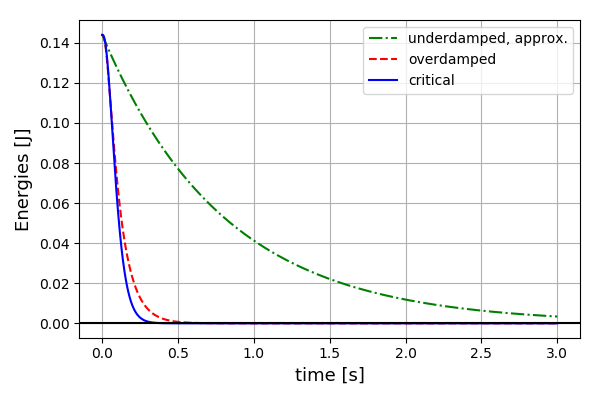
\includegraphics{DampedEnergy.png}
\caption{Fig. 6: Energy of damped oscillations}
\end{figure}

    The critical case is the one for which the energy decays the fastest on
the figure, and in all cases (all other things being equal) as well. In
some engineering problems like the ones I was mentioning before,
removing energy as fast as possible is a desirable quality.

    \hypertarget{quality-factor-q-value-of-an-oscillator}{%
\section{\texorpdfstring{Quality factor (`\(Q\)-value') of an
oscillator}{Quality factor (`Q-value') of an oscillator}}\label{quality-factor-q-value-of-an-oscillator}}

\hypertarget{definition}{%
\subsection{Definition}\label{definition}}

In many other engineering cases, we want a system to require as little
driving as possible, for energy saving purposes for example. If that is
indeed what one wants, the damping has to be as weak as possible. In
this case, the \emph{quality} of the system will therefore be measured
by the ratio
\[ Q = \frac{\textrm{tendency to oscillate}}{\textrm{tendency to damp}}. \]
Now, there is no scientific definition of what these ``tendencies'' are.
But in the lightly damped oscillator (the only one, the \(Q\)-factor
applies to), oscillations last longer when \(\gamma \ll 2\omega_0\).
Therefore, a high ``quality'' (as defined by those for whom this is a
quality\ldots{}) is achieved when
\[ \boxed{Q = \frac{\omega_0}\gamma}. \]

With this definition, the pseudo-angular frequency can be written
\[\omega_d^2 = \omega_0^2\left(1 - \frac1{4Q^2}\right).\]

\(Q\) is called the \emph{quality factor}, \(Q\)\emph{-factor} of
\(Q\)\emph{-value} of the oscillator. In the case I used throughout this
set of notes, \(Q \approx 12\). It can the thought of as a measure of
the number of oscillations (in radians) an oscillator can achieve within
one lifetime. Indeed, define \(\tau = 1/\gamma\) as the lifetime, and
\(n = \tau/T_0\) the number of natural cycles achieved in one lifetime;
then \(Q = 2\pi n\).

    You can verify it on the figures of lightly damped oscillations in this
chapter: we have \(\gamma^{-1} = \tau \approx 0.8\) s, during which you
see the oscillator perform almost two full cycles. \(2\pi \approx 6\), 2
cycles \(\times\) 2\(\pi \approx 12\approx Q\).

It works because \(Q\) is high enough to say that \(T_0 \approx T_d\).
For most practiucal matters, this is the case.

    Fig. 2.7 of King (reproduced here) shows a few examples of oscillators
with different \(b\) parameters, and their corresponding \(Q\) values.

\begin{figure}
\centering
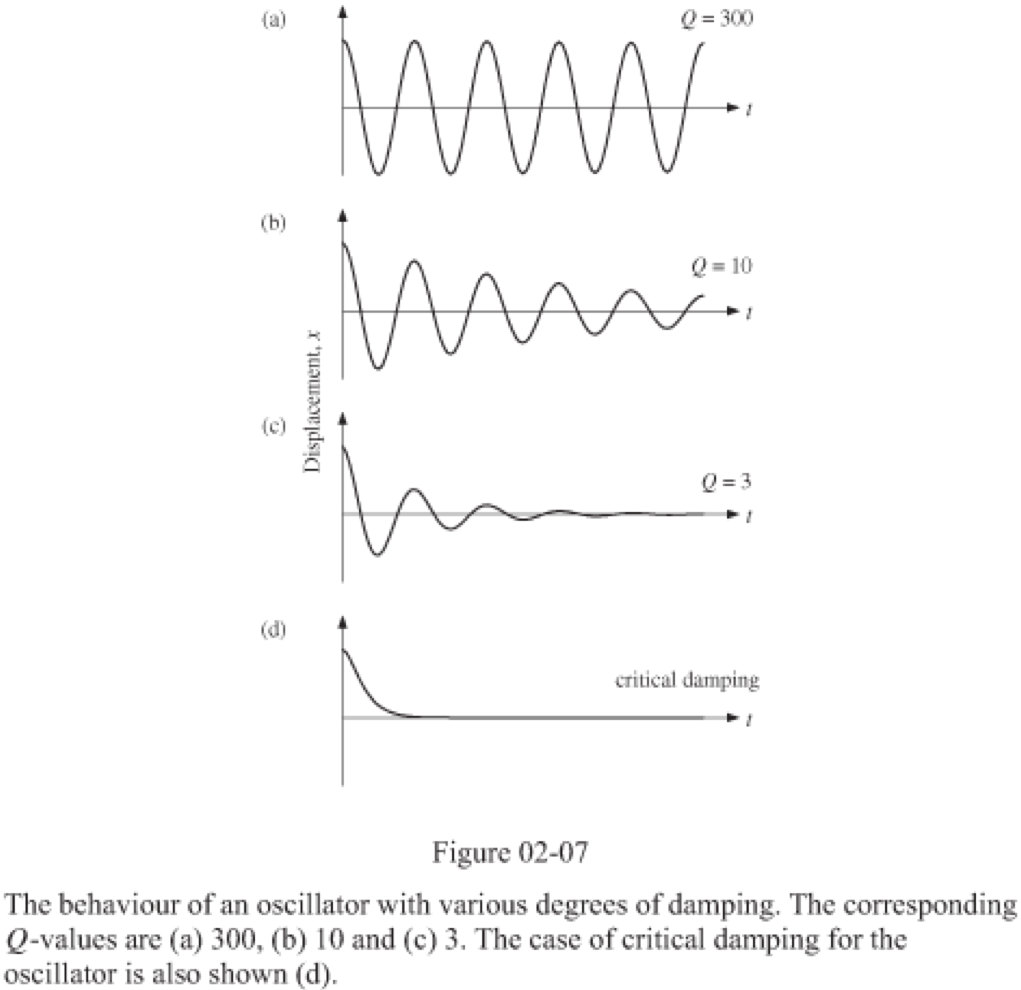
\includegraphics{Q-valuz.png}
\caption{King 2.7: Q-values}
\end{figure}

    \hypertarget{energetic-interpretation}{%
\subsection{Energetic interpretation}\label{energetic-interpretation}}

The quality factor also has an interpretation of how vigorously the
damping removes mechanical energy from the system. Indeed, let
\(E_n = E_0\exp(-\gamma t)\) be the mechanical energy in the system at a
given time \(t\). One pseudo-period later, the mechanical energy will be
\(E_{n+1} = E_0\exp(-\gamma(t+T_d))\).

    The mechanical energy lost in the system during a pseudo-period,
relative to how much energy there was at the beginning of the
pseudo-period, is therefore equal to
\[ \frac{E_{n} - E_{n+1}}{E_n} = \frac{\exp(-\gamma t) - \exp(-\gamma(t+T_d))}{\exp(-\gamma t)} = 1 - \exp(-\gamma T_d).\]

Recall that if \(\varepsilon \ll 1\), then
\(\exp(\varepsilon) = 1 + \varepsilon + O(\varepsilon^2) \approx 1 + \varepsilon\)
(Taylor expansion). Therefore, for a pretty lightly damped oscillator
(\(\gamma \ll \omega_0\), \(Q \gg 1\)),
\[ \frac{E_{n} - E_{n+1}}{E_n} \approx \gamma T_d = \frac{2\pi}{Q}.\]

This was the energy lost \emph{during one (pseudo-)cycle}. The energy
lost \emph{during one (pseudo-)radian} is therefore \(1/Q\). In other
words, a possible interpretation of \(Q\) is
\[ Q  = \frac{\textrm{energy stored in the oscillator}}{\textrm{energy dissipated one radian later}}. \]

    \hypertarget{some-values}{%
\subsection{Some values}\label{some-values}}

Taken from King's Table 2.1.

\begin{longtable}[]{@{}cc@{}}
\toprule
Oscillatory system & Typical value of Q\tabularnewline
\midrule
\endhead
Paper weight suspended on a rubber band & 10\tabularnewline
Clock pendulum & 75\tabularnewline
Electrical LRC circuit & 200\tabularnewline
Plucked violin string & 1,000\tabularnewline
Microwave cavity oscillator & 10,000\tabularnewline
Quartz crystal & 1,000,000\tabularnewline
\bottomrule
\end{longtable}

    \hypertarget{damped-electrical-oscillations-the-lrc-circuit}{%
\section{Damped Electrical Oscillations: the LRC
circuit}\label{damped-electrical-oscillations-the-lrc-circuit}}

See Fig. 2.8 of King attached: we add a resistor (resistance \(R\)) in
series to the circuit we saw in the first chapter, which adds damping to
the system.

\begin{figure}
\centering
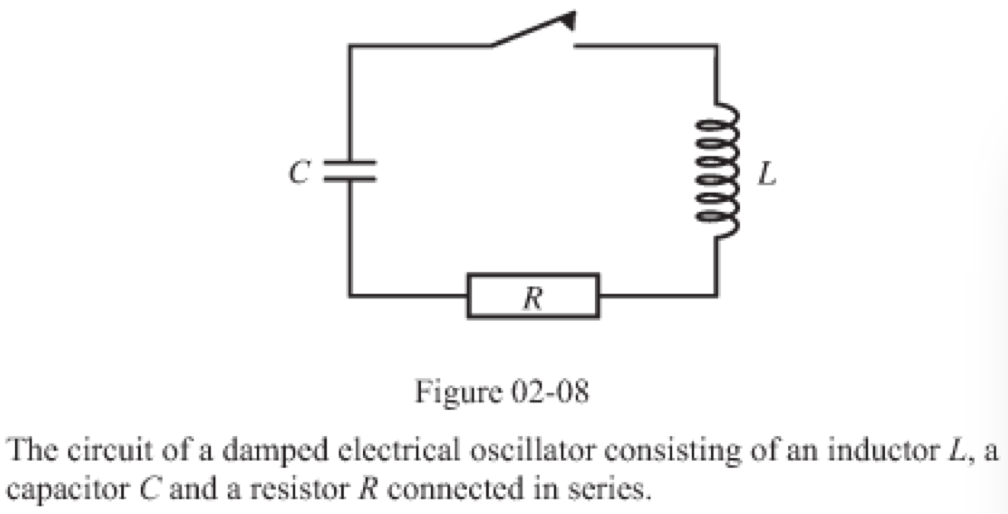
\includegraphics{LRC.png}
\caption{King 2.8: The LRC circuit}
\end{figure}

    Like in the chapter on SHOs, we will draw an analogy between the
spring+mass system and the LRC circuit by simply deriving the equation
for the DHO, and the rest will follow.

Recall that the equivalent of Newton's second law to derive the equation
for an electric circuit is Kirchhoff's law, i.e., all voltages sum up to
zero. Here are the voltages of each component at any instant:

\begin{itemize}
\tightlist
\item
  capacitor: \(V_C = q/C\),
\item
  inductor: \(V_L = L\dot I = L\ddot q\), and
\item
  resistor: \(V_R = RI = R\dot q\).
\end{itemize}

Therefore, because the equivalent of \(\dot x\) is \(\dot q\) here, the
equivalent of \(b\) is now \(R\).

    Kirchoff's law is now written
\[ L\ddot q + R\dot q + q/C = 0 \quad \Rightarrow \quad \ddot q + \gamma\dot q + \omega_0^2 q = 0, \]
after division by \(L\) and with \(\gamma = R/L\) and
\(\omega_0^2 = 1/LC\).

    We can now complete the table, which I started in Chapter 1 on SHOs:

\begin{longtable}[]{@{}cc@{}}
\toprule
\begin{minipage}[b]{0.47\columnwidth}\centering
Mass + spring + damping\strut
\end{minipage} & \begin{minipage}[b]{0.47\columnwidth}\centering
LRC circuit\strut
\end{minipage}\tabularnewline
\midrule
\endhead
\begin{minipage}[t]{0.47\columnwidth}\centering
\(x\)\strut
\end{minipage} & \begin{minipage}[t]{0.47\columnwidth}\centering
\(q\)\strut
\end{minipage}\tabularnewline
\begin{minipage}[t]{0.47\columnwidth}\centering
\(v\)\strut
\end{minipage} & \begin{minipage}[t]{0.47\columnwidth}\centering
\(I\)\strut
\end{minipage}\tabularnewline
\begin{minipage}[t]{0.47\columnwidth}\centering
\(m\)\strut
\end{minipage} & \begin{minipage}[t]{0.47\columnwidth}\centering
\(L\)\strut
\end{minipage}\tabularnewline
\begin{minipage}[t]{0.47\columnwidth}\centering
\(k\)\strut
\end{minipage} & \begin{minipage}[t]{0.47\columnwidth}\centering
\(1/C\)\strut
\end{minipage}\tabularnewline
\begin{minipage}[t]{0.47\columnwidth}\centering
\(\omega_0^2=k/m\)\strut
\end{minipage} & \begin{minipage}[t]{0.47\columnwidth}\centering
\(\omega_0^2=1/(LC)\)\strut
\end{minipage}\tabularnewline
\begin{minipage}[t]{0.47\columnwidth}\centering
KE \(K=mv^2/2\)\strut
\end{minipage} & \begin{minipage}[t]{0.47\columnwidth}\centering
Magnetic energy \(LI^2/2\)\strut
\end{minipage}\tabularnewline
\begin{minipage}[t]{0.47\columnwidth}\centering
PE \(U=kA^2/2\)\strut
\end{minipage} & \begin{minipage}[t]{0.47\columnwidth}\centering
Electrostatic energy \(CV_C^2/2\)\strut
\end{minipage}\tabularnewline
\begin{minipage}[t]{0.47\columnwidth}\centering
\(b\)\strut
\end{minipage} & \begin{minipage}[t]{0.47\columnwidth}\centering
\(R\)\strut
\end{minipage}\tabularnewline
\begin{minipage}[t]{0.47\columnwidth}\centering
\(\gamma=b/m\)\strut
\end{minipage} & \begin{minipage}[t]{0.47\columnwidth}\centering
\(\gamma=R/L\)\strut
\end{minipage}\tabularnewline
\begin{minipage}[t]{0.47\columnwidth}\centering
\(\omega_d^2=\frac1m\left(k-\frac{b^2}{4m}\right)\)\strut
\end{minipage} & \begin{minipage}[t]{0.47\columnwidth}\centering
\(\omega_d^2=\frac1L\left(\frac1C-\frac{R^2}{4L}\right)\)\strut
\end{minipage}\tabularnewline
\begin{minipage}[t]{0.47\columnwidth}\centering
\(Q=\frac{\sqrt{km}}b\)\strut
\end{minipage} & \begin{minipage}[t]{0.47\columnwidth}\centering
\(Q=\frac1R\sqrt{\frac{L}{C}}\)\strut
\end{minipage}\tabularnewline
\bottomrule
\end{longtable}

    Equations are generic, the physics is in the parameters.


    % Add a bibliography block to the postdoc
    
    
    
    \end{document}
